% --------------------------------------------------------------------------
% Formatvorlage für Diplomarbeiten der FHWT
% --------------------------------------------------------------------------
% 	Angelehnt an die Word-Vorlage von Herrn Stührenberg
% 	Download unter http://www.atlando.de/fhwt.htm
%
% 	erstellt von Stefan Macke. 22.10.2007
% 	http://blog.stefan-macke.de
%   
%   Genutzt und angepasst auf utf8 von Johannes Dielmann 

% Meta-Informationen -------------------------------------------------------
%	Informationen über das Dokument, wie z.B. Titel, Autor, Matrikelnr. etc
%	werden in der Datei _Meta.tex definiert und können danach global
%	verwendet werden.
% --------------------------------------------------------------------------
% Informationen ------------------------------------------------------------
% 	Definition von globalen Parametern, die im gesamten Dokument verwendet
% 	werden können (z.B auf dem Deckblatt etc.).
% --------------------------------------------------------------------------
\newcommand{\titel}{\"Ubersetzen von Schrittmotorbefehlen}
\newcommand{\untertitel}{Entwurf eines Hardware\"ubersetzers}
\newcommand{\art}{Praxisbericht}
\newcommand{\fachgebiet}{Mess- und Sensortechnik}
\newcommand{\autor}{Johannes Dielmann}
\newcommand{\studienbereich}{Technik}
\newcommand{\matrikelnr}{515956}
\newcommand{\erstgutachter}{Prof. Dr. Carstens-Behrens}
\newcommand{\zweitgutachter}{Prof. Dr. }
\newcommand{\jahr}{2012}

% Eigene Befehle und typographische Auszeichnungen für diese
\newcommand{\todo}[1]{\textbf{\textsc{\textcolor{red}{(TODO: #1)}}}}

\newcommand{\AutorZ}[1]{\textsc{#1}}
\newcommand{\Autor}[1]{\AutorZ{\citeauthor{#1}}}

\newcommand{\NeuerBegriff}[1]{\textbf{#1}}

\newcommand{\Fachbegriff}[1]{\colorbox{hellblau}{#1}}
\newcommand{\Prozess}[1]{\textit{#1}}
\newcommand{\Webservice}[1]{\textit{#1}}

\newcommand{\Eingabe}[1]{\texttt{#1}}
\newcommand{\Code}[1]{\texttt{\colorbox{hellgelb}{\textcolor{colIdentifier}{#1}}}}
\newcommand{\Datei}[1]{\texttt{\colorbox{hellgelb}{#1}}}

\newcommand{\Datentyp}[1]{\textsf{#1}}
\newcommand{\XMLElement}[1]{\textsf{#1}}


% Abkürzungen mit korrektem Leerraum
\newcommand{\vgl}{Vgl.\ }
\newcommand{\ua}{\mbox{u.\,a.\ }}
\newcommand{\zB}{\mbox{z.\,B.\ }}
\newcommand{\bs}{$\backslash$}



% Dokumentenkopf -----------------------------------------------------------
% 	Diese Vorlage basiert auf "scrreprt" aus dem koma-script.
%	Die Option draft sollte beim fertigen Dokument ausgeschaltet werden.
% --------------------------------------------------------------------------
\documentclass[
	11pt,					% Schriftgröße
	DIV10,
	german,					% für Umlaute, Silbentrennung etc.
	a4paper,         		% Papierformat
	oneside,				% einseitiges Dokument
	titlepage,				% es wird eine Titelseite verwendet
	final					% Status des Dokuments (final/draft)
]{scrreprt}

% Benötigte Packages -------------------------------------------------------
%	Weitere Packages, die benötigt werden, sind in die Datei Packages.tex
%	"ausgelagert", um die Vorlage möglichst übersichtlich zu halten.
% --------------------------------------------------------------------------
% Anpassung des Seitenlayouts ----------------------------------------------
% 	siehe Seitenstil.tex
% --------------------------------------------------------------------------
\usepackage[
	automark,			% Kapitelangaben in Kopfzeile automatisch erstellen
	headsepline,		% Trennlinie unter Kopfzeile
	ilines				% Trennlinie linksbündig ausrichten
]{scrpage2}


% Anpassung an Landessprache -----------------------------------------------
% 	Verwendet globale Option german siehe \documentclass
% --------------------------------------------------------------------------
\usepackage{babel}


% Umlaute ------------------------------------------------------------------
% 	Umlaute/Sonderzeichen wie äüöß direkt im Quelltext verwenden (CodePage).
%		Erlaubt automatische Trennung von Worten mit Umlauten.
% --------------------------------------------------------------------------
\usepackage[utf8]{inputenc}
\usepackage[T1]{fontenc}
\usepackage{textcomp} % Euro-Zeichen etc.

% Grafiken -----------------------------------------------------------------
% 	Einbinden von EPS-Grafiken [draft oder final]
% 	Option [draft] bindet Bilder nicht ein - auch globale Option
% --------------------------------------------------------------------------
\usepackage[dvips,final]{graphicx}
\graphicspath{{Bilder/}} % Dort liegen die Bilder des Dokuments

% Befehle aus AMSTeX für mathematische Symbole z.B. \boldsymbol \mathbb ----
\usepackage{amsmath,amsfonts}


% Weitere Zeichen z.B. \textcelsius \textordmasculine \textsurd \textonehalf 
% \texteuro \texttimes \textdiv ... aus textcomp.sty
% siehe >>Schnell ans Ziel mit \LaTeXe<< von Jörg Knappen
% (Oldenbourg, München und Wien 1997, ISBN 3-486-24199-0)
% \usepackage{tccompat}
	

% Für Index-Ausgabe; \printindex -------------------------------------------
\usepackage{makeidx}


% Einfache Definition der Zeilenabstände und Seitenränder etc. -------------
\usepackage{setspace}
\usepackage{geometry}


% Symbolverzeichnis --------------------------------------------------------
% 	Symbolverzeichnisse bequem erstellen, beruht auf MakeIndex.
% 		makeindex.exe %Name%.nlo -s nomencl.ist -o %Name%.nls
% 	erzeugt dann das Verzeichnis. Dieser Befehl kann z.B. im TeXnicCenter
%		als Postprozessor eingetragen werden, damit er nicht ständig manuell
%		ausgeführt werden muss.
%		Die Definitionen sind ausgegliedert in die Datei Abkuerzungen.tex.
% --------------------------------------------------------------------------
\usepackage[intoc]{nomencl}
  \let\abbrev\nomenclature
  \renewcommand{\nomname}{Abkürzungsverzeichnis}
  \setlength{\nomlabelwidth}{.25\hsize}
  \renewcommand{\nomlabel}[1]{#1 \dotfill}
  \setlength{\nomitemsep}{-\parsep}


% Zum Umfließen von Bildern -------------------------------------------------
\usepackage{floatflt}


% Zum Einbinden von Programmcode --------------------------------------------
\usepackage{listings}
\usepackage{xcolor} 
\definecolor{hellgelb}{rgb}{1,1,0.9}
\definecolor{colKeys}{rgb}{0,0,1}
\definecolor{colIdentifier}{rgb}{0,0,0}
\definecolor{colComments}{rgb}{1,0,0}
\definecolor{colString}{rgb}{0,0.5,0}
\lstset{%
    float=hbp,%
    basicstyle=\texttt\small, %
    identifierstyle=\color{colIdentifier}, %
    keywordstyle=\color{colKeys}, %
    stringstyle=\color{colString}, %
    commentstyle=\color{colComments}, %
    columns=flexible, %
    tabsize=8, %
    frame=single, %
    extendedchars=true, %
    showspaces=false, %
    showstringspaces=false, %
    numbers=left, %
    numberstyle=\tiny, %
    breaklines=true, %
    backgroundcolor=\color{hellgelb}, %
    breakautoindent=true, %
%    captionpos=b%
}

% Lange URLs umbrechen etc. -------------------------------------------------
\usepackage{url}


% Wichtig für korrekte Zitierweise ------------------------------------------
\usepackage[square]{natbib}
% Quellenangaben in eckige Klammern fassen ---------------------------------
\bibpunct{[}{]}{;}{a}{}{,~}


%\usepackage{jurabib}
%\jurabibsetup{authorformat=smallcaps,% Autor in Kapitälchen              
%              %authorformat=year,
%              authorformat=citationreversed,% Im Zitat Vorname vorne
%              authorformat=indexed,% Autor in Index
%              authorformat=and,% Autoren mit "," und "und" abgetrennt
%              authorformat=firstnotreversed,%
%              authorformat=reducedifibidem,% Bei Verweis nur Nachname. 
%              %superscriptedition=all,% Auflage hochgestellt
%              %citefull=first,% Erstzitat voll
%              titleformat=italic,              
%              titleformat=all,
%              titleformat=colonsep,% Doppelpunkt zwischen Aut. u. Titel
%              ibidem=strict,% Ebenda pro Doppelseite
%              see,% Das zweite Argument ist optional für "Vgl." etc.
%              commabeforerest,% Komma vor Seitenzahl
%              %howcited=compare,%
%              %bibformat=ibidem,% Strich bei widerholtem Autor in BIB.
%              commabeforerest,
%              bibformat=compress,
%              pages=always,
%              %pages=format,% S. wird vorweggesetzt
%              crossref=long,% Querverweise in voller Länge
%              square,% eckige Klammern bei Zitaten
%              %oxford,
%              %chicago,
%}
%
%\AddTo\bibsgerman{% 
%\jblookforgender%
%\renewcommand*{\ibidemname}{Ebenda}%
%\renewcommand*{\ibidemmidname}{ebenda}% 
%\renewcommand*{\bibjtsep}{In: }% Vor Zeitschriften 
%\renewcommand*{\bibbtsep}{In: }% Vor Buchtitel
%\renewcommand*{\incollinname}{In: }%Nicht so ganz sauber. 
%\renewcommand*{\bibatsep}{.}% Nach Titel
%\renewcommand*{\bibbdsep}{}%Vor Datum 
%\renewcommand*{\jbaensep}{.}%
%\renewcommand*{\bibprdelim}{)}% Klammer bei Zeitschriftjahr rechts
%\renewcommand*{\bibpldelim}{(}% Klammer bei Zeitschriftjahr links
%\renewcommand*{\biblnfont}{\textsc}% Nachamen Autor im BIB
%\renewcommand*{\bibelnfont}{\textsc}% Nachamen Hg. im BIB
%\renewcommand*{\bibfnfont}{\textsc}% Vorn. Autor im BIB
%\renewcommand*{\bibefnfont}{\textsc}% Vorn. Hg. im BIB
%\renewcommand*{\jbcitationyearformat}[1]{#1}% Komma zwischen Autor und Jahr entfernen
%\def\herename{hier: }%
%\jbfirstcitepageranges% Format: S. x--z, hier y.  
%\renewcommand\bibidemSfname{\raisebox{.2em}{\rule{2.em}{.2pt}}~}%
%\renewcommand\bibidemsfname{\raisebox{.2em}{\rule{2.em}{.2pt}}~}%
%\renewcommand\bibidemPfname{\raisebox{.2em}{\rule{2.em}{.2pt}}~}%
%\renewcommand\bibidempfname{\raisebox{.2em}{\rule{2.em}{.2pt}}~}%
%\renewcommand\bibidemSmname{\raisebox{.2em}{\rule{2.em}{.2pt}}~}%
%\renewcommand\bibidemsmname{\raisebox{.2em}{\rule{2.em}{.2pt}}~}%
%\renewcommand\bibidemPmname{\raisebox{.2em}{\rule{2.em}{.2pt}}~}%
%\renewcommand\bibidempmname{\raisebox{.2em}{\rule{2.em}{.2pt}}~}%
%\renewcommand\idemSfname{Dies.}%
%\renewcommand\idemsfname{dies.}%
%\renewcommand\idemPfname{Dies.}%
%\renewcommand\idempfname{dies.}%
%\renewcommand\idemSmname{Ders.}%
%\renewcommand\idemsmname{ders.}%
%\renewcommand\idemPmname{Dies.}%
%\renewcommand\idempmname{dies.}%
%\renewcommand{\jbannoteformat}[1]{{\footnotesize\begin{quote}#1\end{quote}}}
%}%


%% PDF-Optionen -------------------------------------------------------------
\usepackage[
bookmarks,
bookmarksopen=true,
pdftitle={\titel},
pdfauthor={\autor},
pdfcreator={\autor},
pdfsubject={\titel},
pdfkeywords={\titel},
colorlinks=true,
linkcolor=blue, % einfache interne Verknüpfungen
anchorcolor=black,% Ankertext
citecolor=blue, % Verweise auf Literaturverzeichniseinträge im Text
filecolor=blue, % Verknüpfungen, die lokale Dateien öffnen
menucolor=red, % Acrobat-Menüpunkte
urlcolor=blue, 
%linkcolor=black, % einfache interne Verknüpfungen
%anchorcolor=black,% Ankertext
%citecolor=black, % Verweise auf Literaturverzeichniseinträge im Text
%filecolor=black, % Verknüpfungen, die lokale Dateien öffnen
%menucolor=black, % Acrobat-Menüpunkte
%urlcolor=black, 
backref,
%pagebackref,
plainpages=false,% zur korrekten Erstellung der Bookmarks
pdfpagelabels,% zur korrekten Erstellung der Bookmarks
hypertexnames=false,% zur korrekten Erstellung der Bookmarks
%linktocpage % Seitenzahlen anstatt Text im Inhaltsverzeichnis verlinken
]{hyperref}

% Zum fortlaufenden Durchnummerieren der Fußnoten ---------------------------
\usepackage{chngcntr}


% Aliase für Zitate
% \defcitealias{WPProzess}{Wikipedia:~Prozess}

%\usepackage{minitoc}

% für lange Tabellen
\usepackage{longtable}
\usepackage{array}
\usepackage{ragged2e}
\usepackage{lscape}

%Spaltendefinition rechtsbündig mit definierter Breite
\newcolumntype{w}[1]{>{\raggedleft\hspace{0pt}}p{#1}}

% Formatierung von Listen ändern
\usepackage{paralist}
% \setdefaultleftmargin{2.5em}{2.2em}{1.87em}{1.7em}{1em}{1em}

% Anhangsverzeichnis
%\makeatletter% --> De-TeX-FAQ
%\newcommand*{\maintoc}{% Hauptinhaltsverzeichnis
%\begingroup
%\@fileswfalse% kein neues Verzeichnis öffnen
%\renewcommand*{\appendixattoc}{% Trennanweisung im Inhaltsverzeichnis
%\value{tocdepth}=-10000 % lokal tocdepth auf sehr kleinen Wert setzen
%}%
%\tableofcontents% Verzeichnis ausgeben
%\endgroup
%}
%\newcommand*{\appendixtoc}{% Anhangsinhaltsverzeichnis
%\begingroup
%\edef\@alltocdepth{\the\value{tocdepth}}% tocdepth merken
%\setcounter{tocdepth}{-10000}% Keine Verzeichniseinträge
%\renewcommand*{\contentsname}{% Verzeichnisname ändern
%Verzeichnis der Anh\"ange}%
%\renewcommand*{\appendixattoc}{% Trennanweisung im Inhaltsverzeichnis
%\setcounter{tocdepth}{\@alltocdepth}% tocdepth wiederherstellen
%}%
%\tableofcontents% Verzeichnis ausgeben
%\setcounter{tocdepth}{\@alltocdepth}% tocdepth wiederherstellen
%\endgroup
%}
%\newcommand*{\appendixattoc}
%\g@addto@macro\appendix{% \appendix erweitern
%\if@openright\cleardoublepage\else\clearpage\fi% Neue Seite
%\addcontentsline{toc}{chapter}{\appendixname}% Eintrag ins Hauptverzeichnis
%\addtocontents{toc}{\protect\appendixattoc}% Trennanweisung in die toc-Datei
%}
%\makeatother


% Erstellung eines Index und Abkürzungsverzeichnisses aktivieren -----------
\makeindex
\makenomenclature


% Kopf- und Fußzeilen, Seitenränder etc. -----------------------------------
% Zeilenabstand ------------------------------------------------------------
\onehalfspacing


% Seitenr�nder -------------------------------------------------------------
%\geometry{paper=a4paper,left=30mm,right=40mm,top=10mm,bottom=65mm}
\geometry{paper=a4paper,left=35mm,right=35mm,top=30mm}


% Kopf- und Fu�zeilen ------------------------------------------------------
\pagestyle{scrheadings}

% Kopf- und Fu�zeile auch auf Kapitelanfangsseiten -------------------------
\renewcommand*{\chapterpagestyle}{scrheadings}

% Schriftform der Kopfzeile ------------------------------------------------
\renewcommand{\headfont}{%
\normalfont
}

% Kopfzeile ----------------------------------------------------------------
\ihead{\large{\textsc{\titel}}\\	\small{\untertitel} \\[2ex] \textit{\headmark}}
\chead{}
\ohead{
\includegraphics[scale=0.25]{RAC_Logo.jpg}}
%
\setlength{\headheight}{21mm} % H�he der Kopfzeile
\setheadwidth[0pt]{textwithmarginpar} % Kopfzeile �ber den Text hinaus verbreitern
\setheadsepline[text]{0.4pt} % Trennlinie unter Kopfzeile

% Fu�zeile -----------------------------------------------------------------
\ifoot{\copyright\ \autor}
\cfoot{}
\ofoot{\pagemark}


% erzeugt ein wenig mehr Platz hinter einem Punkt --------------------------
\frenchspacing 

% Schusterjungen und Hurenkinder vermeiden
\clubpenalty = 10000
\widowpenalty = 10000 
\displaywidowpenalty = 10000


% Quellcode-Ausgabe formatieren --------------------------------------------
\lstset{numbers=left, numberstyle=\tiny, numbersep=5pt, breaklines=true}
\lstset{emph={square}, emphstyle=\color{red}, emph={[2]root,base}, emphstyle={[2]\color{blue}}}

% Fu�noten fortlaufend durchnummerieren ------------------------------------
\counterwithout{footnote}{chapter}


% Eigene Definitionen für Silbentrennung
\hyphenation{Laser-er-fass-ungs-system Haupt-ein-satz-ge-bie-te}


% Das eigentliche Dokument -------------------------------------------------
%	Der eigentliche Inhalt des Dokuments beginnt hier. Die einzelnen Seiten
%	und Kapitel werden in eigene Dateien ausgelagert und hier nur inkludiert.
% --------------------------------------------------------------------------
\begin{document}

% auch subsubsection nummerieren
\setcounter{secnumdepth}{3}
\setcounter{tocdepth}{3}

\ofoot{}
\thispagestyle{plain}
\begin{titlepage}

\begin{center}

%\huge{\textbf{\textsc{Vorläufige Arbeitskopie!}}}\\[1.5ex]
\huge{\textbf{\textsc{\titel}}}\\[1.5ex]
\LARGE{\textbf{\untertitel}}\\[4ex]
\LARGE{\textbf{\art}}\\[1.5ex]
\Large{im Fachgebiet \fachgebiet}\\[6ex]


\includegraphics[scale=0.6]{RAC_Logo.jpg}\\[3ex]

\normalsize
\begin{tabular}{w{5.4cm}p{6cm}}\\
 vorgelegt von:	 & \quad \autor\\[1.2ex]
 Geburtsdatum:	 & \quad 10. Januar 1984\\ [1.2ex]
 Geburtsort:	 & \quad Kirchen\\ [1.2ex]
 %Studienbereich: & \quad \fachgebiet\\[1.2ex]
 Matrikelnummer: & \quad \matrikelnr\\[1.2ex]
 Erstgutachter:  & \quad \erstgutachter\\[3ex]
 %Zweitgutachter: & \quad \zweitgutachter\\[3ex]
\end{tabular}

\copyright\ \jahr\\[1.5ex]

\end{center}

\singlespacing
\small
\noindent Dieses Werk einschließlich seiner Teile ist \textbf{urheberrechtlich geschützt}. Jede Verwertung außerhalb der engen Grenzen des Urheberrechtgesetzes ist ohne Zustimmung des Autors unzulässig und strafbar. Das gilt insbesondere für Vervielfältigungen, Übersetzungen, Mikroverfilmungen sowie die Einspeicherung und Verarbeitung in elektronischen Systemen.

\end{titlepage}

%\section*{Zusammenfassung}
\label{sec:Zusammenfassung}
\todo{besser schreiben!} Im Praxisprojekt wurde eine gegebene Aufgabe selbstständig umgesetz. Dabei wurde Hardware unter anderem in Form von Platinenlayouts entwickelt, benötigte Bauteile recherchiert und bestellt, der Aufbau verändert und verbessert. Es wurde Software entwickelt und auftrende Probleme gelöst.

\section*{Abstract}
\label{sec:Abstract}
\todo{WTH is an abstact??}

\ofoot{\pagemark}

% Seitennummerierung -------------------------------------------------------
%	Vor dem Hauptteil werden die Seiten in großen römischen Ziffern 
%	nummeriert...
% --------------------------------------------------------------------------
\pagenumbering{Roman}
%\maintoc
\tableofcontents								% Inhaltsverzeichnis

% Abkürzungsverzeichnis ----------------------------------------------------
%\nomenclature{SCSI}{Small Computer System Interface}
%\nomenclature{ASCII}{American Standard Code for Information Interchange}
%\nomenclature{CAD}{Computer Aided Design}
%\nomenclature{CF}{Compact Flash}
%\nomenclature{LCD}{Liquid Crystal Display}
%\nomenclature{RS}{Recommended Standard}
%\nomenclature{IC}{Integrated Cuircuit}
%\nomenclature{CPU}{Central Processing Unit}
%\nomenclature{ADC}{Analog Digital Convertor}
%\nomenclature{DAC}{Digital Analog Convertor}
%\nomenclature{DIL}{Dual in Line Package}
%\nomenclature{AVRISP}{AVR in System Programmer}
%\nomenclature{USB}{Universal Serial Bus}
%\nomenclature{ISR}{Interrupt Service Routine}
%\nomenclature{UART}{Universal Asynchronous Receiver Transmitter}				
\printnomenclature
\label{sec:Glossar}

\listoffigures						% Abbildungsverzeichnis
\listoftables						% Tabellenverzeichnis
\renewcommand{\lstlistlistingname}{Codeverzeichnis}
\lstlistoflistings					% Listings-Verzeichnis

% ...danach in normalen arabischen Ziffern ---------------------------------
\clearpage
\pagenumbering{arabic}
% Inhalt -------------------------------------------------------------------
%	Hier können jetzt die einzelnen Kapitel inkludiert werden. Sie müssen
%	in den entsprechenden .TEX-Dateien vorliegen. Die Dateinamen können
% 	natürlich angepasst werden.
% --------------------------------------------------------------------------
\chapter{Einleitung}
\label{cha:Einleitung}

\todo {Klarstellen der Begrifflichkeiten}
In der \todo{CAD erklären} \Fachbegriff{CAD-Entwicklung} kommt es vor das für ein real existierendes Objekt eine Erweiterung konstruiert werden muss. Um die Erweiterung sinnvoll konstruieren zu können müssen dazu die Abmessungen des Objektes möglichst genau bekannt sein. Das übertragen der Abmessungen, kann insbesondere für komplexe Objekte, sehr aufwendig sein.
Abhilfe soll ein Laserscanner schaffen der das Objekt aus mehreren Richtungen vermisst und aus diesen Informationen ein genaues 3D-Modell davon generiert. 

\section{Motivation}
\label{sec:Motivation}
Mit dem Aufbau aus RapidForm2004, Lasererfassungssystem VI-900 und Drehtisch sollen auf einfachem Wege 3D-Modelle eines Objektes erzeugt werden. Diese sollen anschließend in einer CAD-Software wie \Fachbegriff{Solidworks} nutzbar sein.\\

\section{Ziel der Arbeit}
\label{sec:ZielDerArbeit}
Die Kommunikation zwischen der Software RapidForm2004 und dem gegebenen Drehtisch soll ermöglicht werden. Dazu werden die ASCII-Befehle der Software mit einem Mikrocontroller ausgewertet und in für den gegeben Schrittmotor verständliche Befehle übersetzt.
Es wird also ein Mikrocontroller mit 2 RS-232 Schnittstellen so programmiert das er die Befehle der Software übersetzen kann. Um den den Drehtisch manuell bedienen zu können und den aktuellen Status zu überprüfen sind noch ein LC-Display und mehrere Bedientaster vorgesehen.\\
Die Ansteuerung des Schrittmotors ist als Einschub für ein 19"-Rack realisiert. Daher wird die Platine für den Mikrocontroller auch als 19"-Einschub realisiert.


\section{Aufbau der Arbeit}
\label{sec:AufbauDerArbeit}
\todo{Ausbauen!} Überblick verschaffen. Kommunikation mit Schrittmotor-Karte von PC aus. Aufbauen des STK500. Einarbeiten in uC Entwicklung. Steuern der Schrittmotor Karte vom uC aus. Erarbeiten der Protokolle (Reverse Engineering). C-Programm zum verstehen eingehender Befehle. Übersetzen der Befehle. Neuer Mikrocontroller. Umgebungs wechsel. LC-Display. Endschalter. Max232. Platinenlayout.


\section{Typographische Konventionen}
\todo{Was hier?}Proin id magna eu sem tincidunt feugiat. Sed tincidunt massa sed eros. Fusce condimentum eros et lectus. Pellentesque lectus tortor, mattis in, dapibus a, lobortis ut, justo. Sed id dolor ut nibh varius ultrices. Quisque tincidunt nisl vel nibh. Suspendisse sodales massa non magna. In porttitor augue nonummy nunc. Nam quis enim quis ante dapibus interdum. Morbi nec neque. Fusce pharetra consectetuer magna. Etiam laoreet, augue nec lacinia ornare, risus purus lobortis erat, eu consequat urna orci vel arcu. Integer cursus, augue sed tempor dapibus, erat tortor rutrum elit, sit amet fermentum purus neque vitae tortor. Donec vulputate, ipsum vel viverra pretium, purus orci mattis nulla, nec tincidunt leo metus sed ipsum. Fusce eget lectus sed lectus molestie tincidunt. Etiam tincidunt urna eget tortor. 		% Motivation und Ziel
\chapter{Begriffe und Komponenten}
\label{cha:Begriffe}
\todo{Besseres Bild! Schema? Bessere Beschriftung!}
\begin{figure}[htb]
\centering
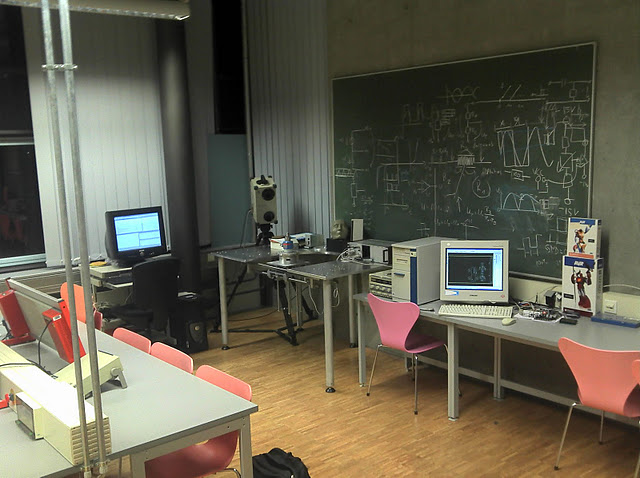
\includegraphics[width=\textwidth]{Uebersicht.jpg}
\caption{Überblick des Arbeitsplatz}
\label{fig:Übersicht}
\end{figure}
\todo{Bessere Überschrift!}
\todo{ Fußnoten für Komponenten, Hersteller und Websites}
\todo{ Komponenten auf Abbildung erwähnen!}
\section{Kopmonenten zur Erfassung}
\subsection{Lasererfassungssystem VI-900}
Das Lasererfassungsystem VI-900 der Firma Minolta besteht aus einem Lasertriangulator und einer Kamera. Das System lässt sich über eine SCSI Schnittstelle ansprechen und konfigurieren. Zur mobilen Nutzung kann das Gerät auch auf der Rückseite bedient werden. Aufgenommene Daten können auf einer CF-Karte gespeichert werden. Im Projekt wurde jedoch lediglich die Ansteuerung via SCSI genutzt.
\subsection{RapidForm2004}

\section{Drehtisch}
Der Drehtisch ist eine Eigenkonstruktion der Werkstatt des RheinAhrCampus. Er besteht aus einer massiven Edelstahl Arbeitsplatte, welche auf 4 Füßen ruht. Aus dieser ist eine \todo{Welche form??} ausgeschnitten. In diesem Ausschnitt befindet sich, auf einem Zweischienensystem gelagert, der Drehtisch. Mit dem Schienensystem lässt der Drehtisch sich in der Vertikalen positionieren. Mit einem Schrittmotor lässt sich der Drehtisch in der Höhe verstellen. Ein weiterer Schrittmotor ist für die Drehung des Tisches zuständig. \todo{Getriebe erklären!}  
\subsection{Schrittmotoren}
\todo{Motoren beschreiben!}
\subsection{Schrittmotorkarten}
Die Ansteurung für den Drehtisch besteht aus einem 19"-Rack. In diesem ist ein ATX-PC-Netzteil verbaut. Außerdem sind 2 Einschubkarten der Firma R+S vorhanden. Die Karten sind sogenannte Stepper-Karten. Diese übernehmen komfortabel die Ansteuerung der beiden Schrittmotoren. Mittels RS-232 Schnittstelle lassen sich die Karten konfigurieren und ansteuern. Die Konfiguration und Ansteuerung erfolgt über einen vorgegeben ASCII Befehlssatz. Außerdem können 2 oder mehr Karten als "Daisy-Chain" zusammengeschaltet werden. 
\todo{Daisy-Chain erklären und Konfiguration genauer beschreiben.}
\section{Mikrocontroller}
\subsection{Entwicklungsumgebung}
\subsection{Entwicklerboard STK500}
Um den eingesetzten Mikrocontroller zu programmieren und die Programmierung zu überprüfen wurde mir das Entwicklerboard STK500 der Firma ATMEL zur Verfügung gestellt. Das Board enthält mehrere Mikrocontroller Steckplätze, 2 Serielle Schnittstellen, 8 Taster, 8 LEDs, 2 Erweiterungsports, ein integriertes Programmiersystem \todo{besserer Name!} und mehrere Jumper zum konfigurieren des Boards.\\
Von den beiden seriellen Schnittstellen kann die eine zur Programmierung des Mikrocontroller verwendet werden. Die andere kann zur Kommunikation mit dem Mikrocontroller genutzt werden.\\
Auf dem Board stehen 5 10 polige Stiftleisten 
\footnote{Eine Stiftleiste (engl. pin header) ist ein Steckverbinder mit mehreren in Reihe angeordneten Stiftkontakten, der auf Leiterplatten in der Elektronik Verwendung findet. Sie hat den Zweck, eine Verbindung mit vielen Kontakten von einer Platine zu einer anderen oder zu peripheren Baugruppen herzustellen, meist mit Hilfe von Flachbandkabeln und Pfostenverbindern oder einer Buchsenleiste. \cite{wiki_pinh} }
zur Verfügung. Diese sind direkt mit dem Mikrocontroller verbunden und können über Flachbandkabel an Peripherie wie z.B. Taster, LED und LC-Displays angeschlossen werden.
\subsection{AVRISP mkII}
	% Begriffe
\chapter{Vorstellung der vorhanden Hardware}
\label{sec:Hardware}
%Die Hardware besteht im wesentlichen aus den Komponenten in Abbildung \ref{fig:Übersicht}.
%\todo{Nummern oder Farben in Bild!}
%\begin{figure}[htb]
%\centering
%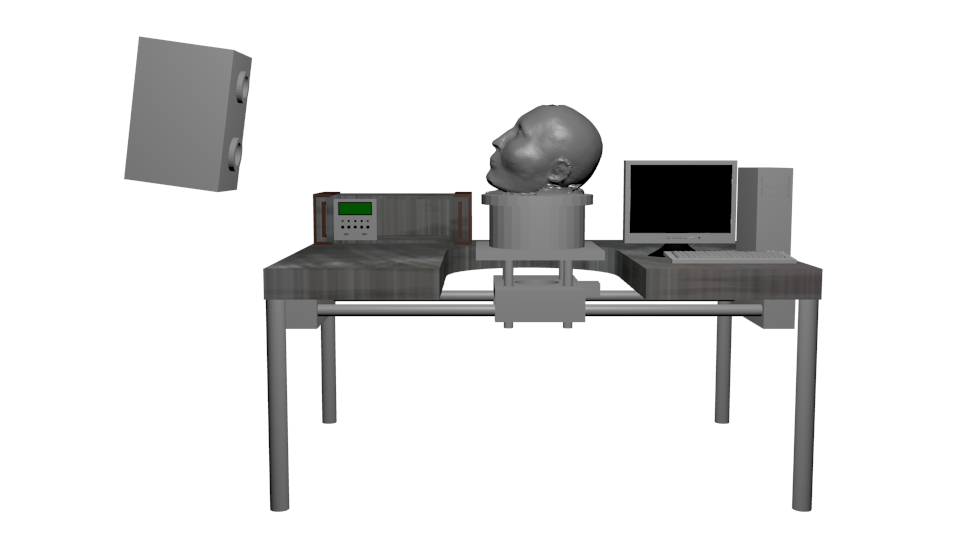
\includegraphics[width=\textwidth]{Blender/Schema_Arbeitsplatz.png}
%\caption{Blick auf den Arbeitsaufbau}
%\label{fig:Übersicht}
%\end{figure}
%\todo{ Komponenten auf Abbildung erwähnen!}

\section{Computer}
\label{sec:Computer}
Zur Verfügung steht ein IBM kompatibler x86 Standard PC mit \\
einer SCSI-Schnittstelle und zwei seriellen RS-232-Schnittstellen. Von denen jedoch nur eine genutzt wird.

\section{3D-Laserscanner VI-900}
\label{sec:VI-900}
\begin{figure}[htb]
\centering
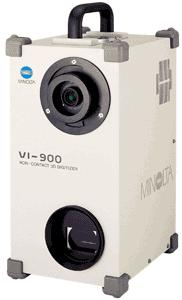
\includegraphics[width=100pt]{vi900-big.jpg}
\caption{VI-900 - 3D-Scanner}
\label{fig:VI900}
\end{figure}
Der 3D-Laserscanner \Fachbegriff{VI-900} der Firma Minolta besteht, wie auf Abbildung \ref{fig:VI900} zu sehen, aus einem \Fachbegriff{Lasertriangulator}(unten) und einer Kamera(oben). Das System lässt sich über eine \Fachbegriff{SCSI}-Schnittstelle ansprechen und konfigurieren. Zur mobilen Nutzung kann das Gerät auch auf der Rückseite bedient werden. Aufgenommene Daten können auf einer \Fachbegriff{CF-Karte} gespeichert werden. Im Projekt wurde jedoch lediglich die direkte Ansteuerung via SCSI genutzt.
\subsection{Lasertriangulator Prinzip}
\label{sec:LaserTri}
Ein Lasertriangulator, wie in Abbildung \ref{fig:LaserTriangulator} zu sehen, besteht aus einem Laser, einem Linsensystem und im einfachsten Fall aus einer Pixeldetektorzeile. Der Laser strahlt auf ein Objekt und je nach Entfernung des Objektes wird das Streulicht unter einem anderen Winkel zurückgestrahlt. Das Streulicht wird durch die Linsen auf den Pixeldetektor abgebildet. Über die Position des Laserspots auf dem Pixeldetektor lässt sich auf die Entfernung des Objektes schließen.\\
Der VI-900 digitalisiert Objekte durch ein Laser-Lichtschnittverfahren. Das vom Objekt reflektierte Licht wird von einer CCD-Flächenkamera erfasst, nach Ermittlung der Distanzwerte (Z-Achse) mittels Laser-Triangulation werden die 3D-Daten erstellt. Der Laserstrahl wird mit Hilfe eines hochpräzisen galvanischen Spiegels über das Objekt projiziert, pro Scan werden 640 x 480 Einzelpunkte erfasst.\cite{Minolta:Einleitung}\\
Die Technischen Daten befinden sich im Anhang in Tabelle \ref{tab:TD_VI-910}
\begin{figure}[htb]
\centering
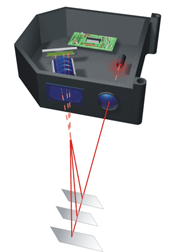
\includegraphics[width=100pt]{Laser-Triangulation.png}
\caption{Prinzip: Laser-Triangulation}
\label{fig:LaserTriangulator}
\end{figure}

\section{Ansteuerung für den Drehtisch}
\label{sec:AnsteuerungDrehtisch}
Die Ansteuerung für den Drehtisch ist in einem 19''-Rack verbaut(siehe Abbildung \ref{fig:19Zoll_Rack}).
\begin{figure}[htb]
\centering
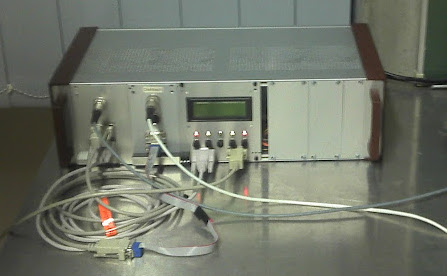
\includegraphics[width=100pt]{19Zoll_Rack}
\caption{Ansteuerung im 19''-Rack}
\label{fig:19Zoll_Rack}
\end{figure}

\subsection{Drehtisch}
\label{sec:Drehtisch}
\begin{figure}[htb]
\centering
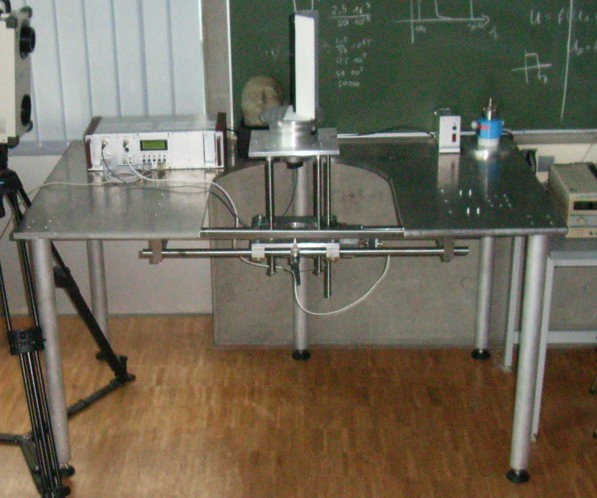
\includegraphics[width=100pt]{Drehtisch}
\caption{Drehtisch}
\label{fig:Drehtisch}
\end{figure}
Der Drehtisch(siehe Abbildung \ref{fig:Übersicht}) ist eine Eigenkonstruktion der Werkstatt des RheinAhrCampus. Er besteht aus einer massiven Edelstahl Arbeitsplatte, welche auf 4 Füßen ruht. Aus dieser ist ein Rechteck mit aufgesetztem Halbkreis ausgeschnitten. In diesem Ausschnitt befindet sich der Drehtisch. Er ist auf einem Schienensystem gelagert. Mit dem Schienensystem kann der Drehtisch in der Vertikalen positioniert werden. Mit einem Schrittmotor lässt sich der Drehtisch zusätzlich in der Höhe verstellen. Die Höhenverstellung wird mit einem \Fachbegriff{Schneckengetriebe} realisiert. Ein weiterer Schrittmotor ist für die Drehung des Tisches zuständig. Der Tisch ist über ein \Fachbegriff{Harmonic-Drive-Getriebe} mit dem Schrittmotor verbunden. Das Übersetzungsverhältnis beträgt 1:50.  
 
\subsection{Spannungsversorgung}
\label{sec:Spannungsv}
Die Schrittmotorkarten werden von einem PC-Netzteil gespeist. Die \Fachbegriff{Logikbausteine} werden mit 5V gespeist, zusätzlich werden die Schrittmotorkarten mit 12V für die Schrittmotoren gespeist. Die Kabel sind direkt an die \todo{Verbindungsleisten} gelötet.\\
Dies verhindert das einfache Ausbauen der Spannungsversorgung und die einfache Erweiterung um neue Einschubkarten.
\subsection{Schrittmotoren}
\label{sec:Schrittmotoren}
\todo{Motoren beschreiben! Technische Daten!}\\
\todo{Schritte, Spannungen. Verdrahtung.}

\subsection{Schrittmotorkarten}
\label{sec:Schrittmotorkarten}
Die Ansteuerung für die Schrittmotoren sind als 19''-Einschübe realisiert. Für jeden Schrittmotor wird ein Einschub benötigt.
Die Einschübe sind Produkte der Firma R+S. Mittels \Fachbegriff{RS-232 Schnittstelle} lassen sich die Karten konfigurieren und ansteuern. Die Konfiguration und Ansteuerung erfolgt über einen vorgegeben 
\Fachbegriff{ASCII}\footnote{Der American Standard Code for Information Interchange (ASCII, alternativ US-ASCII, oft [æski] ausgesprochen) ist eine 7-Bit-Zeichenkodierung\cite{wiki:ASCII}}
 Befehlssatz. Der Befehlssatz befindet sich im Kapitel \ref{sec:A_ASCII_Befehle}. Es können zwei oder mehr Karten als 
\Fachbegriff{Daisy-Chain}\footnote{Als Daisy Chain (englisch, wörtlich „Gänseblümchenkette“) bezeichnet man eine Anzahl von Hardware-Komponenten, welche in Serie miteinander verbunden sind (meist in sogenannten Bussystemen in der Automatisierungstechnik).\cite{wiki:Daisy} } 
in Reihe geschaltet werden.
\subsection{Motorverkabelung}
\label{sec:Motorverkabelung}
Die Schrittmotoren benötigen ein mindestens 4-adriges Kabel. Das Kabel für den Schrittmotor, der für die Rotation zuständig ist, war bereits gefertigt. Ein Kabel zwischen Schrittmotor und Schrittmotorkarte zur Höhenverstellung und für die Endschalter ist nicht vorhanden. 


\subsection{Endschalter}
\label{sec:Endschalter}
Die Schrittmotorkarten unterstützen das Abschalten der Motoren wenn ein sogenannter Endschalter ausgelöst wird. Dies sind im allgemeinen mechanische Schalter die ausgelöst werden wenn der Tisch sich dem Ende des Arbeitsbereiches nähert. Dies verhindert eine Beschädigung des Aufbaus.\\
Im Aufbau sind bereits induktive Endschalter der Firma \textit{Pepperl+Fuchs} verbaut. 
Am Drehtisch ist ein Metallstutzen von ungenügender Länge angebracht. Durch die ungenügende Länge des Metallstutzen würde der Endschalter nicht rechtzeitig ausgelöst werden und der Aufbau des Drehtisches würde beschädigt.


\section{Mikrocontroller}
\label{sec:Mikrocontroller}
Ein \Fachbegriff{Mikrocontroller} vereint, in einem IC, die wichtigsten Komponenten um komplexe technische Probleme leicht lösen zu können. Dazu gehören z.B. CPU, Flash-Speicher, Arbeitsspeicher, Register, Ports, ADC, DAC und mehr. Einen schematischen Überblick über die Komponenten eines Mikrocontrollers bietet das Blockdiagramm in Abbildung \ref{fig:uC_Blockdiagramm}. \\
Für unterschiedliche Aufgaben sind unterschiedliche Mikrocontroller geeignet.\\
Es steht ein ATmega8515 \cite{atmel:8515} im DIL-Gehäuse zur Verfügung. Dieser hat 8 Kbyte Flash, drei externe Interrupts, eine serielle Schnittstelle und kann mit bis zu 16 MHz betrieben werden. 
Dieser ist geeignet um sich in die Programmierung mit \Fachbegriff{C} einzufinden und eine serielle Schnittstelle anzusteuern. \\
Für dieses Projekt sind jedoch zwei serielle Schnittstellen nötig. Der ATmega 324A \cite{atmel:324A} würde diese Voraussetzungen erfüllen, ist jedoch nicht vorhanden. Er ist dem ATmega 8515 recht ähnlich, bietet jedoch die benötigten zwei seriellen Schnittstellen. Des Weiteren hat er 32 Kbyte Flash. 
%Diese wurden aufgrund des recht umfangreichen Programms und der diversen Bibliotheken notwendig.
\begin{figure}[htb]
\centering
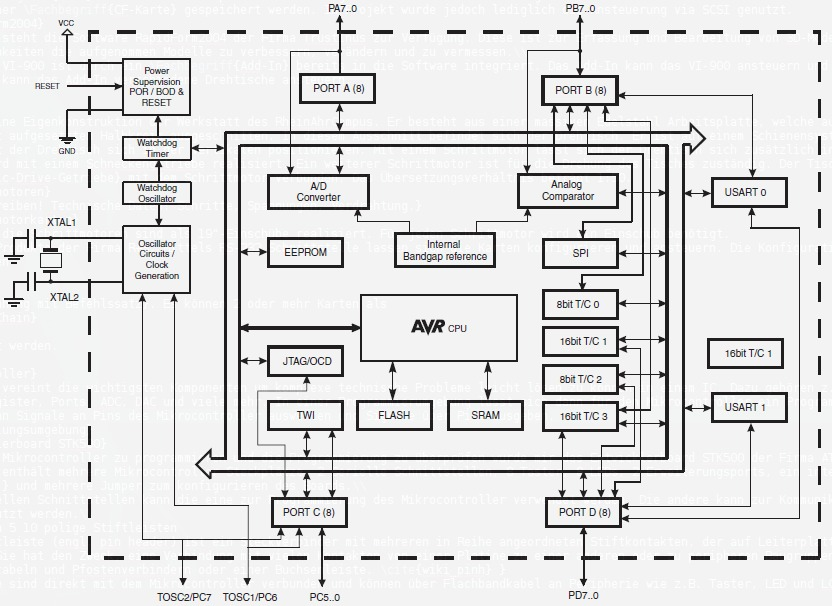
\includegraphics[width=\textwidth]{uC_Block}
\caption{Block Diagram: Mikrocontroller}
\label{fig:uC_Blockdiagramm}
\citep{atmel:ug_324A}
\end{figure}

\subsection{Entwicklerboard STK500}
\label{sec:STK500}
Um den Mikrocontroller zu programmieren und die Programmierung zu überprüfen, soll das \Fachbegriff{Entwicklerboard STK500}(siehe Abbildung \ref{fig:STK500}) der Firma Atmel verwendet werden. Das Board enthält mehrere Mikrocontroller-Steckplätze, 2 serielle Schnittstellen, 8 Taster, 8 LEDs, 2 Erweiterungsports, eine Programmierschnittstelle \Fachbegriff{ISP}\footnote{In System Programmer} und mehrere Jumper zum Konfigurieren des Boards.\\
Von den beiden seriellen Schnittstellen kann die eine zur Programmierung des Mikrocontrollers verwendet werden. Die andere kann zur Kommunikation mit dem Mikrocontroller genutzt werden.\\
Auf dem Board stehen fünf 10 polige Stiftleisten 
zur Verfügung. Diese sind direkt mit den Ports des Mikrocontroller verbunden und können über Flachbandkabel mit \todo{Peripherie} wie z.B. Taster, LED, LC-Displays oder seriellen Schnittstellen verbunden werden.
\begin{figure}[htb]
\centering
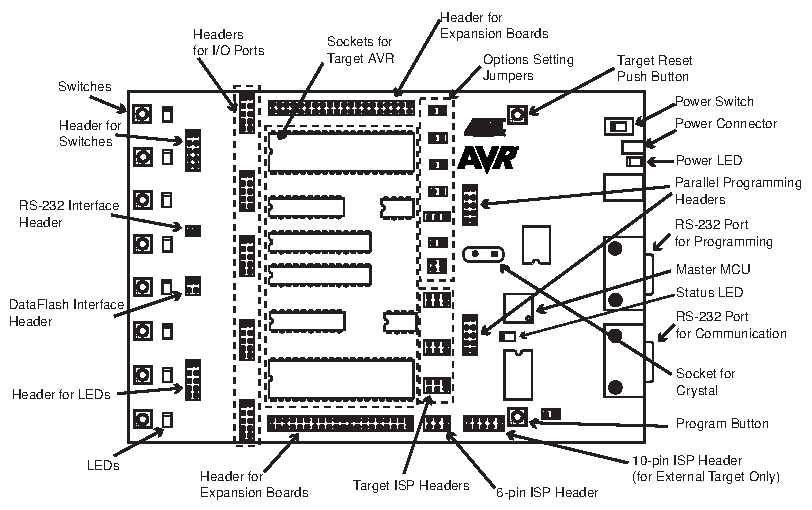
\includegraphics[width=\textwidth]{STK500_Schema.pdf}
\caption{Schema: STK500}
\label{fig:STK500}
\citep{atmel:ug_STK500}
\end{figure}

\subsection{AVRISP mkII}
\label{sec:AVRISP}
Das AVRISP mkII ist ein USB-basiertes \Fachbegriff{In-System-Programmiersystem}. Dieses kann anstelle des RS-232 basierten Programmiersystem des STK500 verwendet werden.\\
Die Übertragungsgeschwindigkeit des AVRISP mkII ist wesentlich höher als die der Seriellen Schnittstelle. 
%Desweiteren wurde der ATmega324A nicht mehr vom STK500 internen ISP unterstützt.\\
Der AVRISP mkII lässt sich einfach an den Programmierport, eine 6-Polige Stiftleiste, des STK500 anschließen.

\subsection{MAX232}
\label{sec:MAX232}
Um die Serielle Schnittstelle am Mikrocontroller nutzen zu können müssen die Spannungspegel auf die des RS-232 Standard gewandelt werden. Dazu befindet sich auf dem STK500 der \Fachbegriff{Pegelwandler} MAX232. 
Dieser wandelt die Spannungspegel des Mikrocontroller(typ. 0 V -- 5 V \Fachbegriff{TTL\footnote{Transistor-Transistor-Logik}}) auf die Spannungspegel des RS-232 Standards (typ. -12 V -- +12 V).
	% Hardwareentwicklung
\chapter{Vorstellung der vorhandenen Software}
\label{cha:Software}

\section{RapidForm2004}
\label{sec:RapidForm}
Zur Erfassung von 3D-Modellen am PC steht die Software RapidForm2004 der Firma INUS Technology Inc. zur Verfügung. Diese ist zur Erfassung und Bearbeitung von 3D-Modellen gedacht. Sie bietet umfangreiche Möglichkeiten die aufgenommenen Modelle zu verbessern, zu verändern, zu vermessen und in verschiedene Formate zu exportieren.\\
Die Ansteuerung des VI-900 ist durch ein \Fachbegriff{Add-In} bereits in die Software integriert. Das Add-In kann den VI-900 ansteuern und die aufgenommenen Daten auslesen. Weiterhin kann das Add-In verschiedene Drehtische ansteuern.

\section{Entwicklungsumgebung}
\label{sec:Entwicklungsumgebung}
Die von Atmel bereitgestellte Entwicklungsumgebung besteht aus einem Editor, dem Compiler und einer Programmiersoftware. Der Editor bietet Komfortfunktionen wie \Fachbegriff{Syntaxhighlighting}, Autovervollständigung und Projektmanagement.

\section{Terminalprogramme}
\label{sec:Terminal}
Als Terminalprogramm zur Kommunikation zwischen Datengeräten über die serielle Schnittstelle steht das Programm "Hypterminal" der Firma Microsoft zur Verfügung.

%\subsection{AVR Studio 5}
%Die von Atmel AVR Studio 5 ist eine von Atmel bereitgestellte Entwicklungsumgebung. Diese scheint jedoch eine fehlerhafte Bibliothek zu enthalten. Die Kombination aus Mikrocontroller ATmega324A und AVR Studio 5 erzeugte nicht nachvollziehbare Probleme. Bei dem selbem Programm und einem anderem Mikrocontroller oder einer anderen Entwicklungsumgebung tauchten keine Fehler auf.
%In der Entwicklungsumgebung Eclipse lies sich der Fehler reproduzieren wenn der Pfad der Atmel Bibliotheken eingestellt wurde. Die WinAVR Bibliotheken und eine selbst kompilierte \Fachbegriff{Toolchain} unter Linux zeigten keine Probleme.\\
%Daher wechselte ich zur \Fachbegriff{Open Source} Entwicklungsumgebung Eclipse. Erst dadurch wurde es möglich erfolgreich zu arbeiten. Außerdem wurde das Projekt dadurch plattformunabhänig und ich nutzte bis auf RapidForm2004 nur noch freie Open Source Software.\\
%\subsection{Eclipse}
%Eclipse ist eine in Java programmierte freie Open Source Entwicklungsumgebung für Java. Sie lässt sich durch \Fachbegriff{Plugins} leicht für viele Sprachen erweitern.\\
%Mit dem CDT-Plugin, dem AVR-Plugin und einer Bibliothek wie z.B. WinAVR für Windows ist Eclipse eine vollwertige Entwicklungsumgebung für Atmel Mikrocontroller. 
%Ergänzt wird diese durch die Programmiersoftware AVR-Dude.\\












	% Softwareentwicklung
\chapter{Fazit und kritische Bewertung}
\label{cha:Fazit}
Lorem ipsum dolor sit amet, consectetuer adipiscing elit. Nulla ac ipsum a metus viverra tempor. Nunc sem. Nulla nec urna eu nibh vehicula convallis. Integer ac turpis. Donec mauris enim, dignissim quis, scelerisque ac, rhoncus id, sapien. Donec turpis felis, cursus in, varius vitae, mollis ac, lorem. Integer a dui sit amet eros nonummy aliquet. Donec egestas adipiscing tellus. Nulla iaculis. Aliquam erat volutpat. Curabitur posuere, eros vitae accumsan semper, risus erat viverra erat, eu vehicula mi leo at elit. Fusce luctus. Fusce vehicula pretium diam. Nunc sed arcu ut erat suscipit fermentum.

Proin id magna eu sem tincidunt feugiat. Sed tincidunt massa sed eros. Fusce condimentum eros et lectus. Pellentesque lectus tortor, mattis in, dapibus a, lobortis ut, justo. Sed id dolor ut nibh varius ultrices. Quisque tincidunt nisl vel nibh. Suspendisse sodales massa non magna. In porttitor augue nonummy nunc. Nam quis enim quis ante dapibus interdum. Morbi nec neque. Fusce pharetra consectetuer magna. Etiam laoreet, augue nec lacinia ornare, risus purus lobortis erat, eu consequat urna orci vel arcu. Integer cursus, augue sed tempor dapibus, erat tortor rutrum elit, sit amet fermentum purus neque vitae tortor. Donec vulputate, ipsum vel viverra pretium, purus orci mattis nulla, nec tincidunt leo metus sed ipsum. Fusce eget lectus sed lectus molestie tincidunt. Etiam tincidunt urna eget tortor.

Sed sit amet magna at lectus interdum blandit. Proin vitae metus eget leo bibendum ornare. Morbi sit amet nisl ac odio accumsan laoreet. Etiam luctus massa vel enim. Vestibulum nulla tellus, viverra at, malesuada vel, volutpat quis, lorem. Vestibulum quis nulla. Curabitur neque nibh, bibendum vel, eleifend sit amet, euismod at, leo. Duis auctor lobortis justo. Donec in tortor vel nibh rutrum pellentesque. Curabitur blandit pede quis neque. Nam sem eros, ornare a, pretium eget, condimentum sed, leo. Curabitur orci felis, elementum eget, aliquet vel, porta id, velit. Etiam justo neque, rhoncus quis, elementum vel, auctor vitae, urna.

				% Fazit und Zukunft

% Literaturverzeichnis -----------------------------------------------------
%	Das Literaturverzeichnis wird aus der Datenbank Bibliographie.bib 
% 	erstellt. Die genaue Verwendung von bibtex wird hier jedoch nicht erklärt.
%	Link: http://de.wikipedia.org/wiki/BibTeX
% --------------------------------------------------------------------------
\bibliography{Bibliographie}		% Aufruf: bibtex FHWTVorlage
\bibliographystyle{natdin}			% DIN-Stil des Literaturverzeichnisses
%\chapter*{Erklärung des Autors}
%\addcontentsline{toc}{chapter}{Erklärung des Autors}
\addchap{Eidesstattliche Erklärung}
Ich versichere hiermit, dass ich meine Diplomarbeit mit dem Thema
\begin{quote}
\textit{\titel} \textit{\untertitel}
\end{quote}
selbständig verfasst und keine anderen als die angegebenen Quellen und Hilfsmittel benutzt habe. Die Arbeit wurde bisher keiner anderen Prüfungsbehörde vorgelegt und auch nicht veröffentlicht.

Die Ergebnisse der Arbeit stehen ausschließlich dem auf dem Deckblatt angeführten Unternehmen zur Verfügung (\textbf{Arbeit mit Sperrvermerk}).

Mir ist bekannt, dass ich meine Diplomarbeit zusammen mit dieser Erklärung fristgemäß nach Vergabe des Themas in dreifacher Ausfertigung und gebunden im Prüfungsamt der FHWT abzugeben oder spätestens mit dem Poststempel des Tages, an dem die Frist abläuft, zu senden habe.\\[6ex]

Vechta, den \today


\rule[-0.2cm]{5cm}{0.5pt}

\textsc{\autor} 
			% Selbständigkeitserklärung 

% Anhang -------------------------------------------------------------------
%		Die Inhalte des Anhangs werden analog zu den Kapiteln inkludiert.
%		Dies geschieht in der Datei Anhang.tex
% --------------------------------------------------------------------------
\begin{appendix}
	\clearpage
	\pagenumbering{roman}
	\chapter{Anhang}
\label{sec:Anhang}

% Rand der Aufzählungen in Tabellen anpassen
\setdefaultleftmargin{1em}{}{}{}{}{}

%\appendixtoc
\section{Schritt für Schritt Anleitung}
\label{sec:StepbyStep}
Eine Schritt für Schritt Anleitung zum vollständigen Scannen und exportieren eines 3D-Objektes.

\begin{longtable}{|>{\RaggedRight}m{5cm}|m{8cm}|} 
\caption{Schritt für Schritt Anleitung} 
\label{tab:StepbyStep}
\\ \hline
%\multicolumn{2}{|c|}{\textbf{Schritt für Schritt Anleitung}}
%\\ \hline 
%\endfirsthead


%\multicolumn{2}{|c|}%
%{{ Fortsetzung }} 
%\\ \hline 
%\endhead

\multicolumn{2}{|l|}%
{{\textbf{Schritt 1 - Einschalten der Schrittmotorsteuerung}}}
\\ \hline
Auf der Rückseite des 19''-Rack befindet sich ein Schalter. Mit diesem kann die Steuerung eingeschaltet werden.
& 
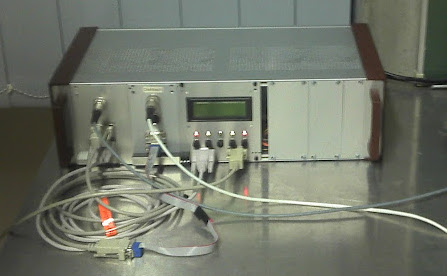
\includegraphics[width=8cm]{19Zoll_Rack}
\\ \hline 

\multicolumn{2}{|l|}%
{{\textbf{Schritt 2 - Einschalten des VI-900}}}
\\ \hline
\multicolumn{2}{|p{13cm}|}%
{Bevor der VI-900 eingeschaltet wird, muss der Erfassungs-PC eingeschaltet werden. Kurz nach dem BIOS wird nach SCSI Geräten gesucht. Zu diesem Zeitpunkt muss der VI-900 eingeschaltet werden.}
\\ \hline 
 
\multicolumn{2}{|l|}%
{{\textbf{Schritt 3 - Einloggen}}}
\\ \hline
\multicolumn{2}{|l|}%
{{Der Benutzername lautet \textbf{Minolta}, das Passwort kann leer bleiben.}}
\\ \hline  
 
\multicolumn{2}{|l|}%
{{\textbf{Schritt 4 - Starten von RapidForm2004}}}
\\ \hline
Auf dem Desktop doppelt auf das Icon \textbf{RapidForm} Icon klicken.
& 
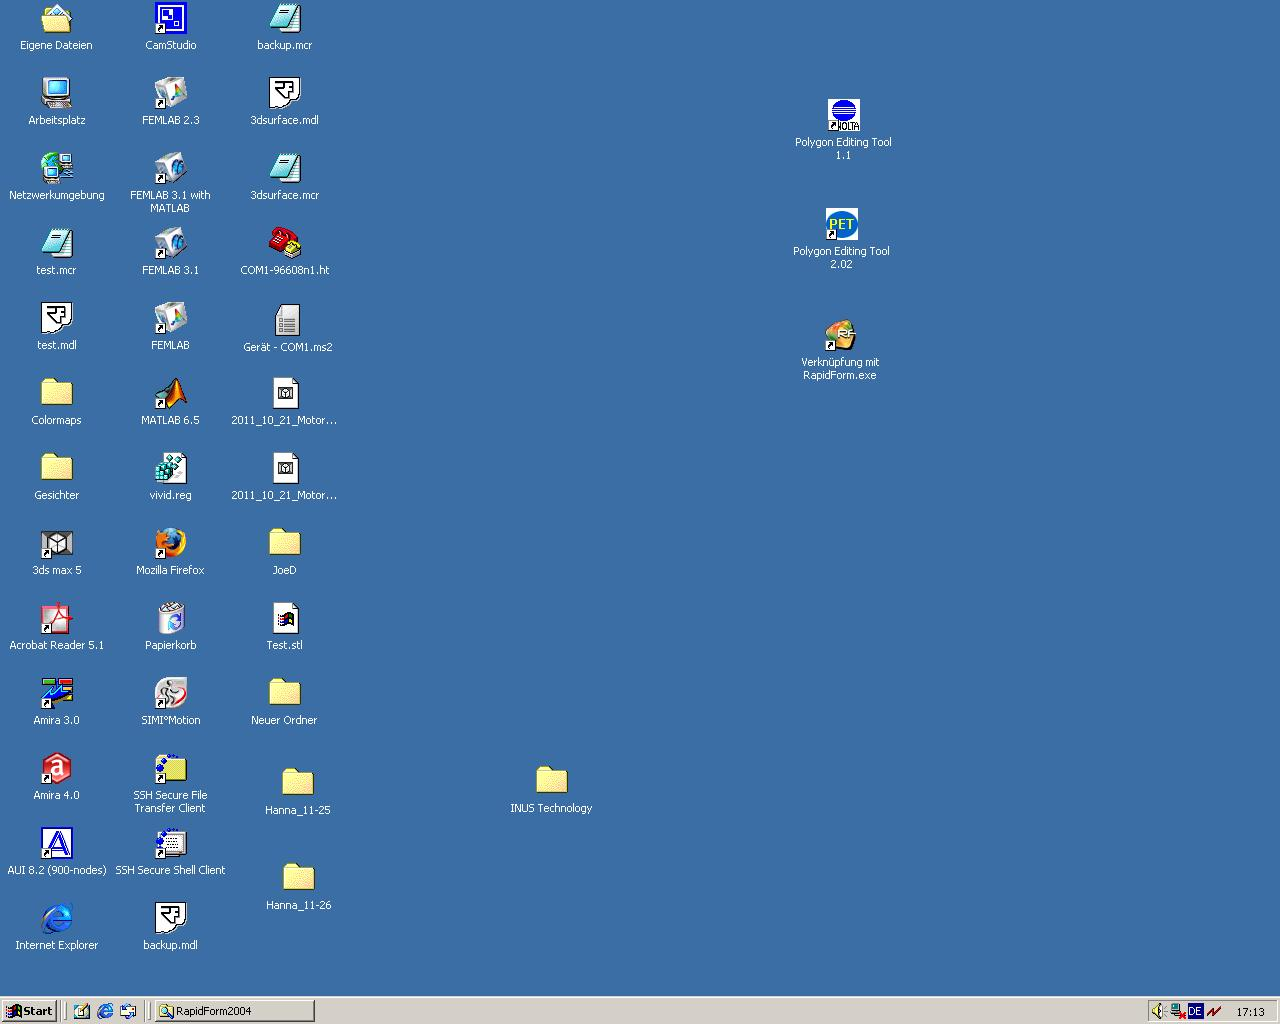
\includegraphics[width=8cm]{Anleitung/1_Desktop}
\\ \hline 

\multicolumn{2}{|l|}%
{{\textbf{Schritt 5 - Oberfläche von RapidForm2004}}}
\\ \hline
Die Oberfläche unterteilt sich in Menü, Werkzeugleisten, Projektbaum und Anzeigefläche.
Je nach dem welche Ansicht in der Anzeigefläche gewählt ist, verändern sich auch das Menü und die Werkzeugleisten. 
& 
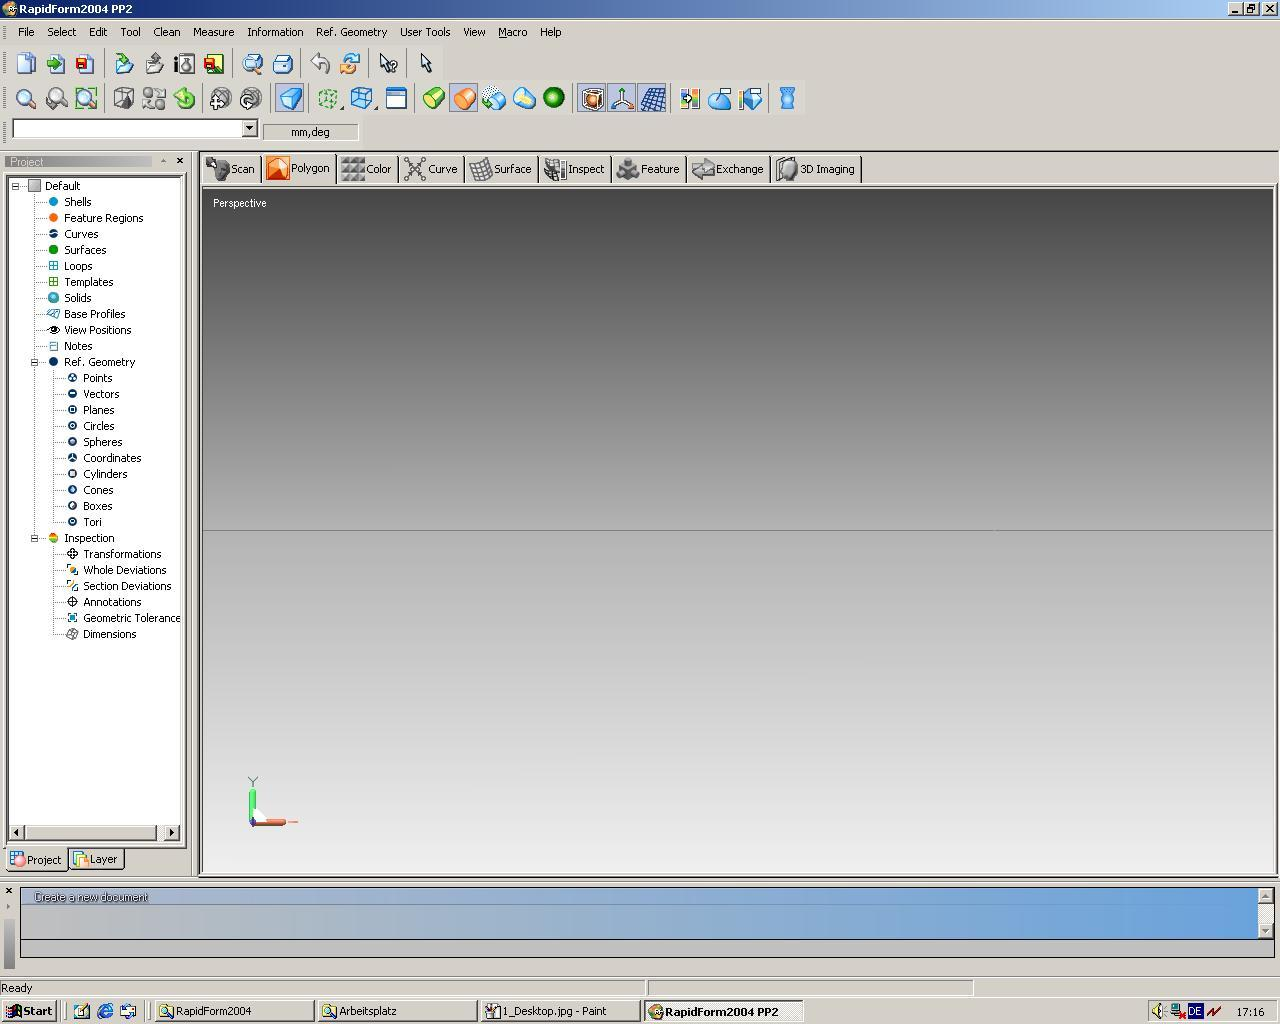
\includegraphics[width=8cm]{Anleitung/2_RapidForm}
\\ \hline  

\multicolumn{2}{|l|}%
{{\textbf{Schritt 6 - Starten des ''ADD-IN''}}}
\\ \hline
In der Menüzeile auf 
\textbf{Macro -> Addins -> Konica Minolta VIVID Direct Control Addin v2.6.11}
klicken.
\todo{Schrittmotor verbinden!}
& 
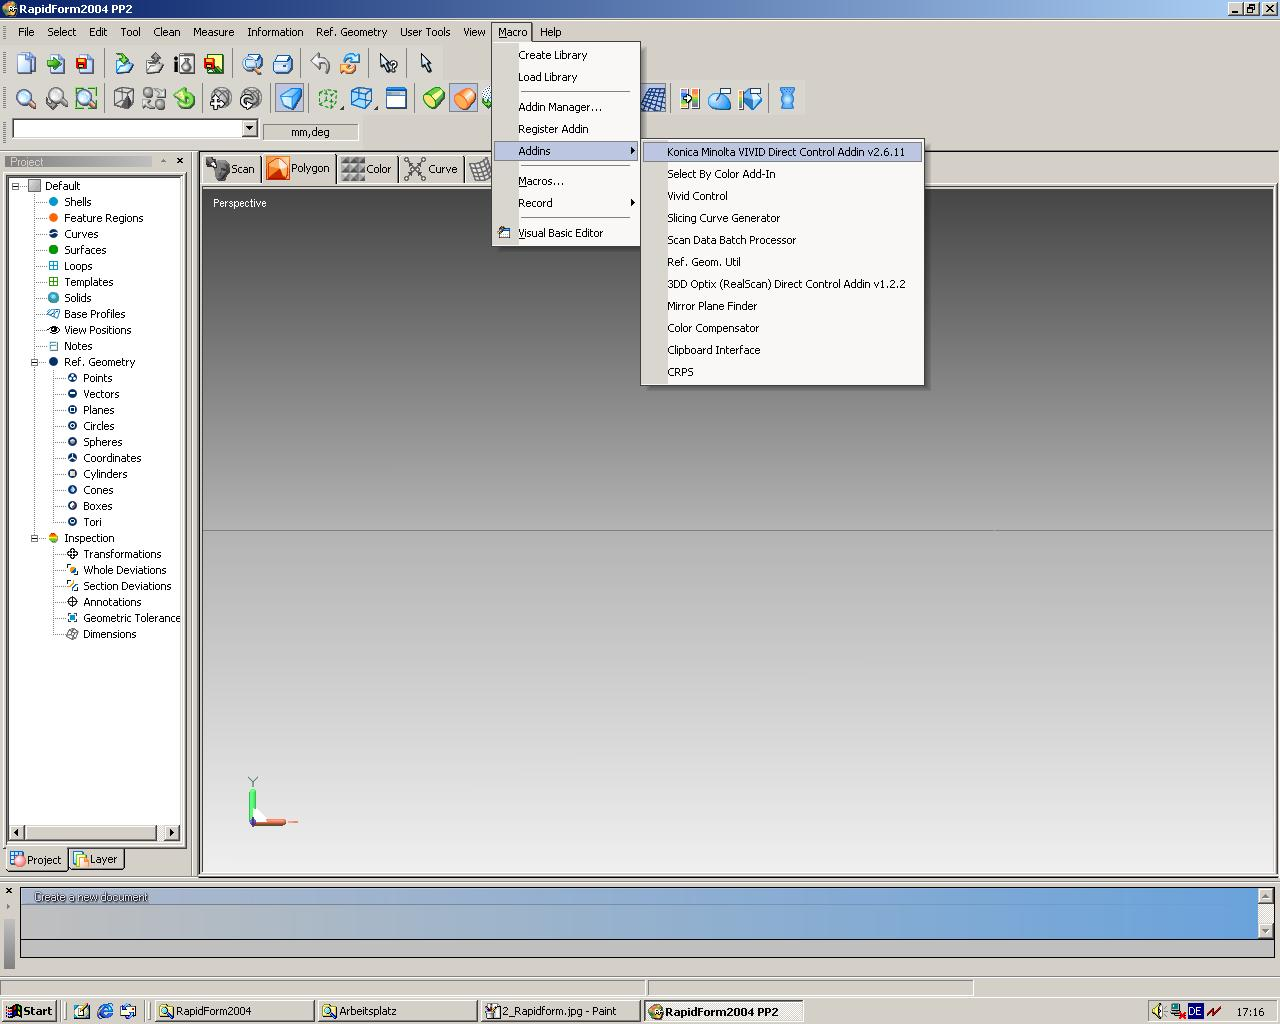
\includegraphics[width=8cm]{Anleitung/3_ADDIN_Menu}
\\ \hline  

\multicolumn{2}{|l|}%
{{\textbf{Schritt 7 - Kalibrieren vorbereiten}}}
\\ \hline
\begin{TippS}Für ein erfolgreiches Zusammenführen der einzelnen Aufnahmen ist die Kalibrierung unerlässlich!\end{TippS}
Auf dem Add-In Panel, unter dem Vorschau Fenster, auf \textbf{Live-Preview} klicken. \linebreak
Das Kalibrierungsblech auf dem Drehtisch positionieren.  \linebreak
Dabei muss der Noppen an der Unterseite des Kalibrierungsblechs in das mittlere Loch des Drehtisches gesteckt werden. Die abgeklebte Seite muss zum VI-900 zeigen.
& 
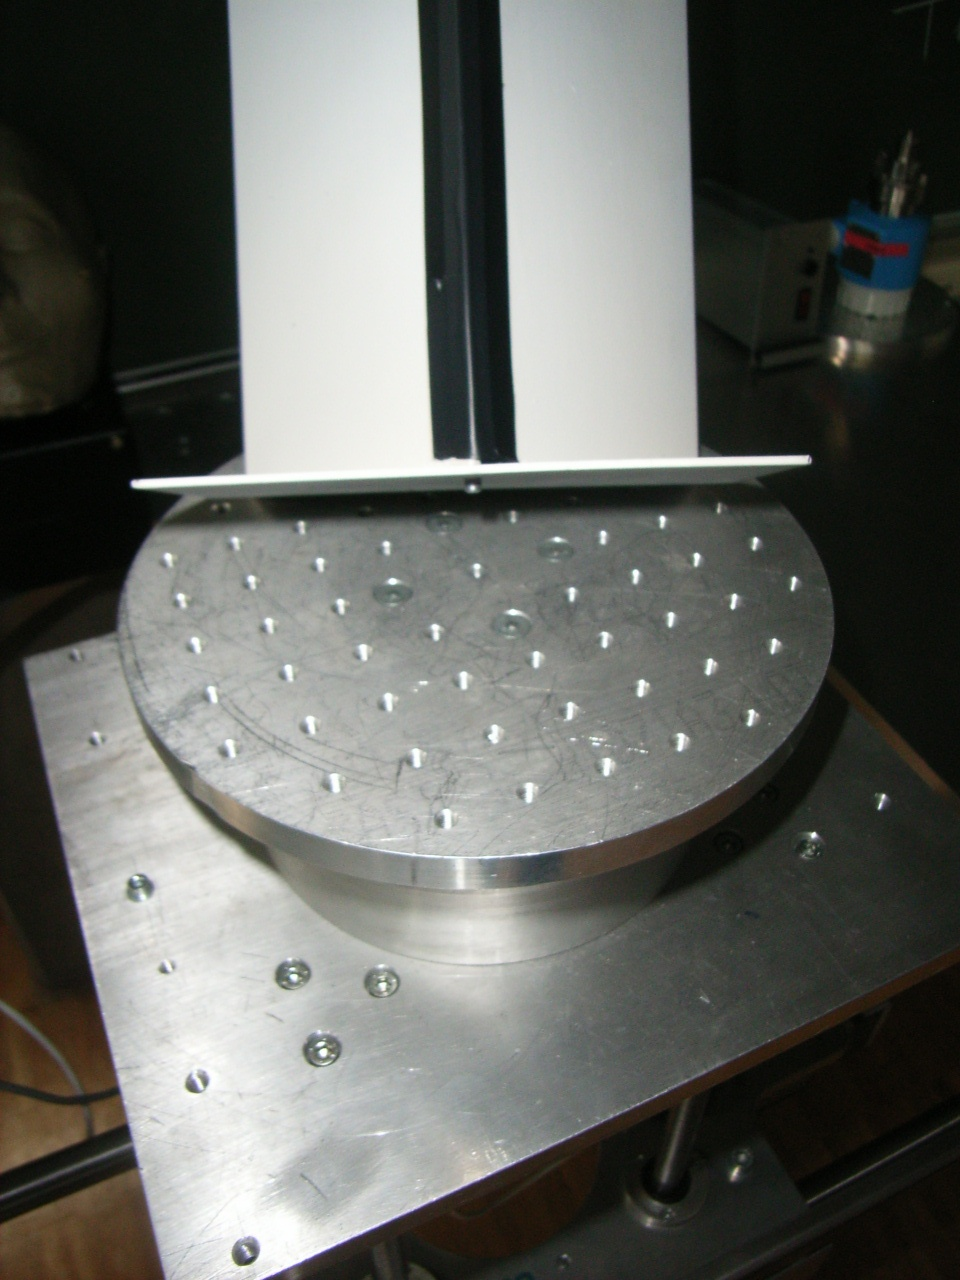
\includegraphics[width=8cm]{Anleitung/4_5_Calibration}
\\ \hline  

\multicolumn{2}{|l|}%
{{\textbf{Schritt 8 - Kalibrieren}}}
\\ \hline
Den Reiter \textbf{VIVID: 1} auswählen.\linebreak
Bei \textbf{Manual Para.} ein Häkchen setzen.\linebreak
Im Feld \textbf{Laser Power} ''23'' eintragen.\linebreak
Auf \textbf{Scan for Calib} klicken.
& 
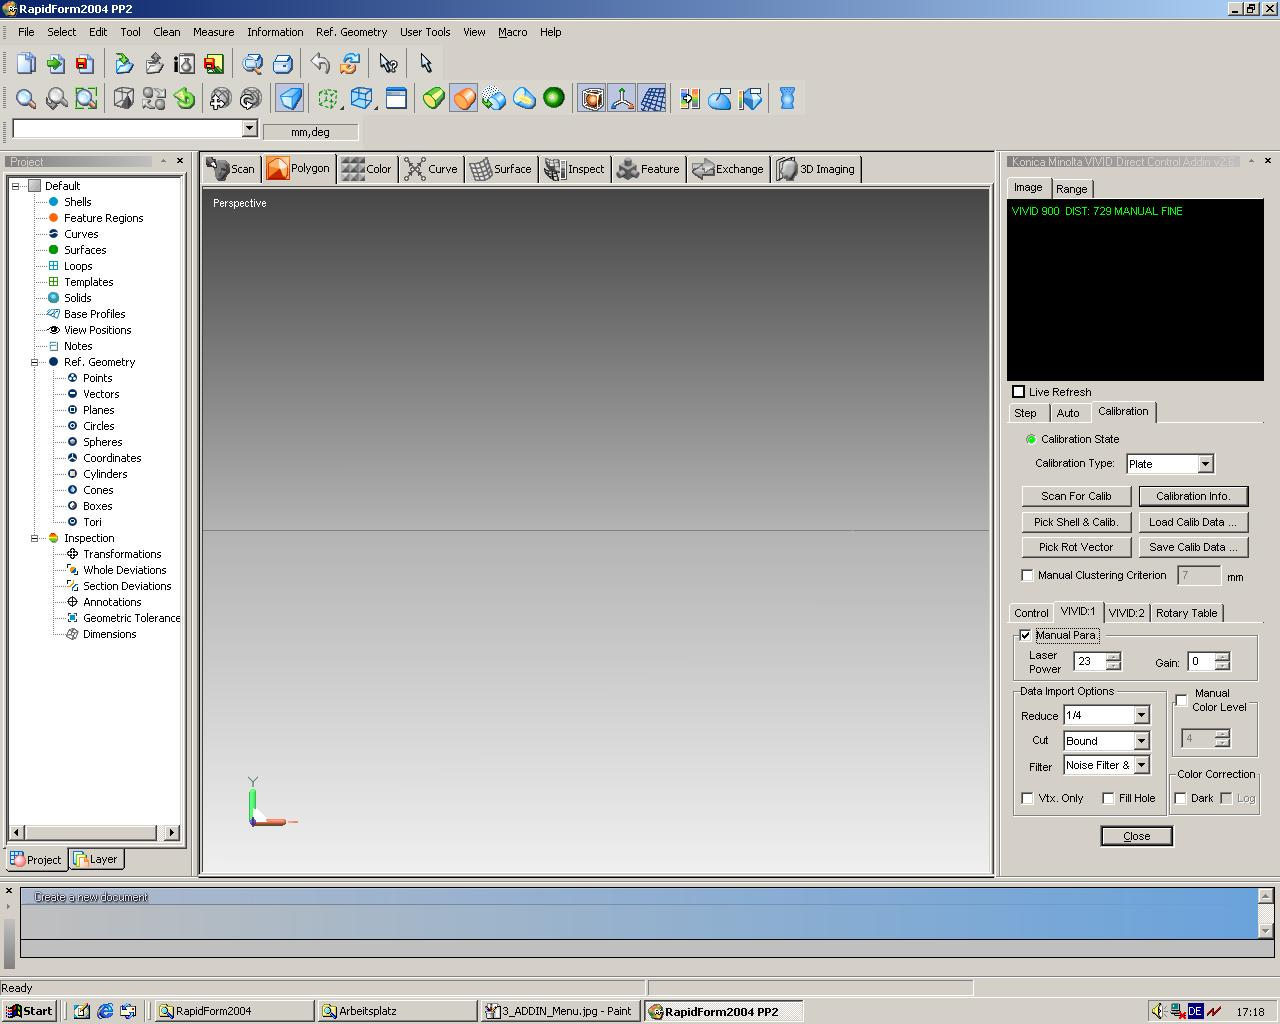
\includegraphics[width=8cm]{Anleitung/4_Calibration}
\\ \hline  

\multicolumn{2}{|l|}%
{{\textbf{Schritt 9 - Kalibrierungsergebnis}}}
\\ \hline
Das Ergebnis sollte ähnlich zu dem in der rechten Abbildung sein. \linebreak
Falls das Add-In einen Fehler ausgibt, muss das Kalibrierungsblech eventuell anders positioniert werden, der Wert im Feld \textbf{Laser Power} verändert werden oder der Fokus manuell eingestellt werden.\linebreak
War die Kalibrierung erfolgreich, können die \emph{Kalibrationsebenen} im \emph{Projektbaum} ausgeblendet werden.
& 
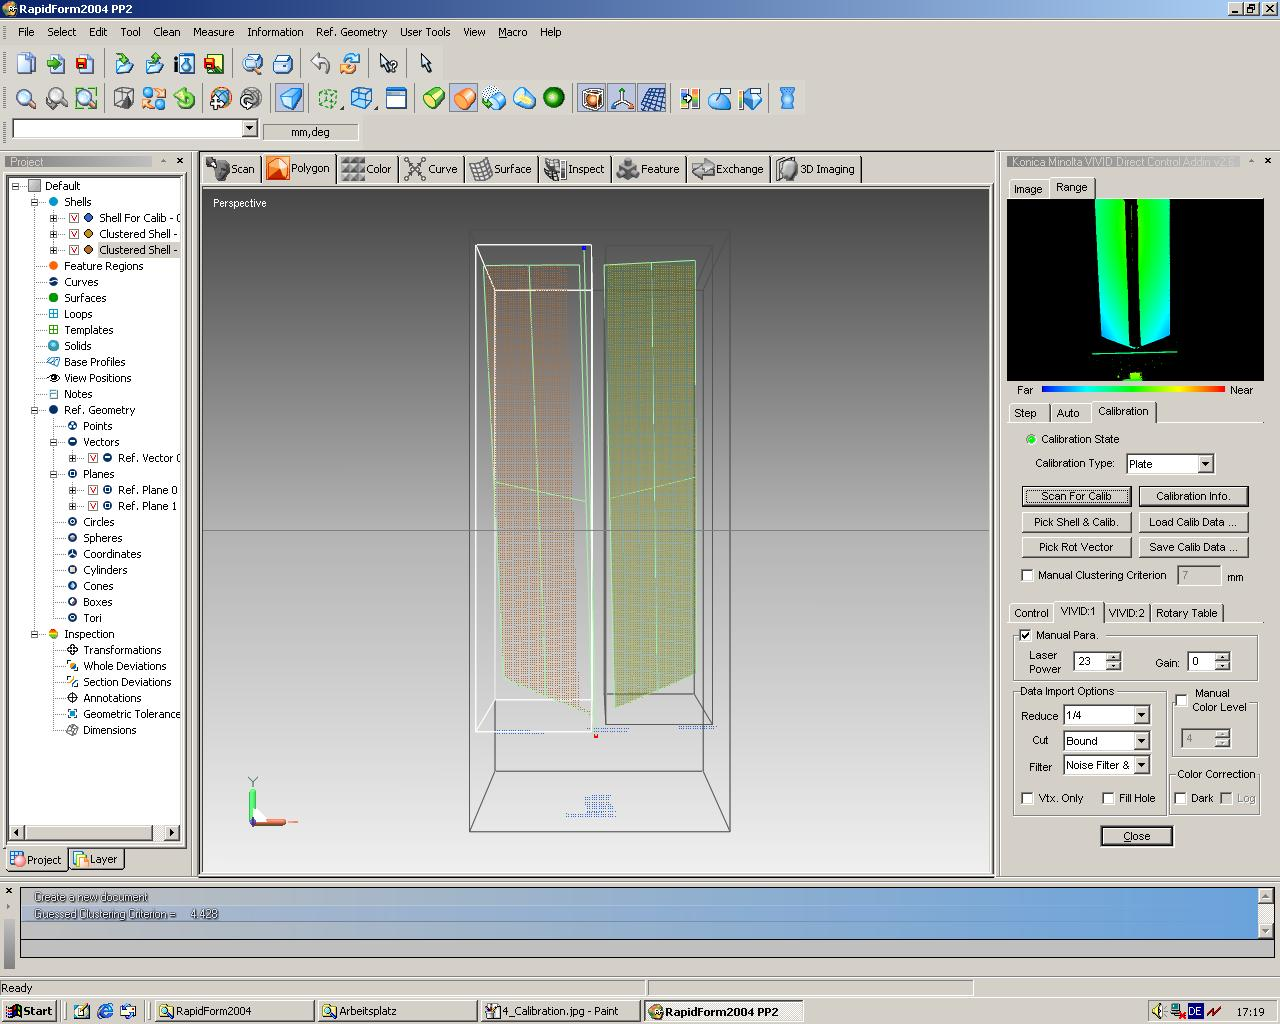
\includegraphics[width=8cm]{Anleitung/4_Calibration_result}
\\ \hline  

\multicolumn{2}{|l|}%
{{\textbf{Schritt 10 - StepScan}}}
\\ \hline
Bei \textbf{Manual Para.} das Häkchen entfernen.\linebreak
Zum Reiter \textbf{Step} wechseln.\linebreak
Bei \textbf{Angle Tag} und \textbf{Rotate Table to next Scan position} Häkchen setzen.\linebreak
Bei \textbf{Init. Align in RF Using Rotary Info.} und \textbf{Auto Accept} die Häkchen entfernen.\linebreak
Bei \textbf{Rotation Step} die gewünschte Drehung in Grad eingeben. \linebreak
''45'', ''60'' und ''90'' sind gute Werte.
& 
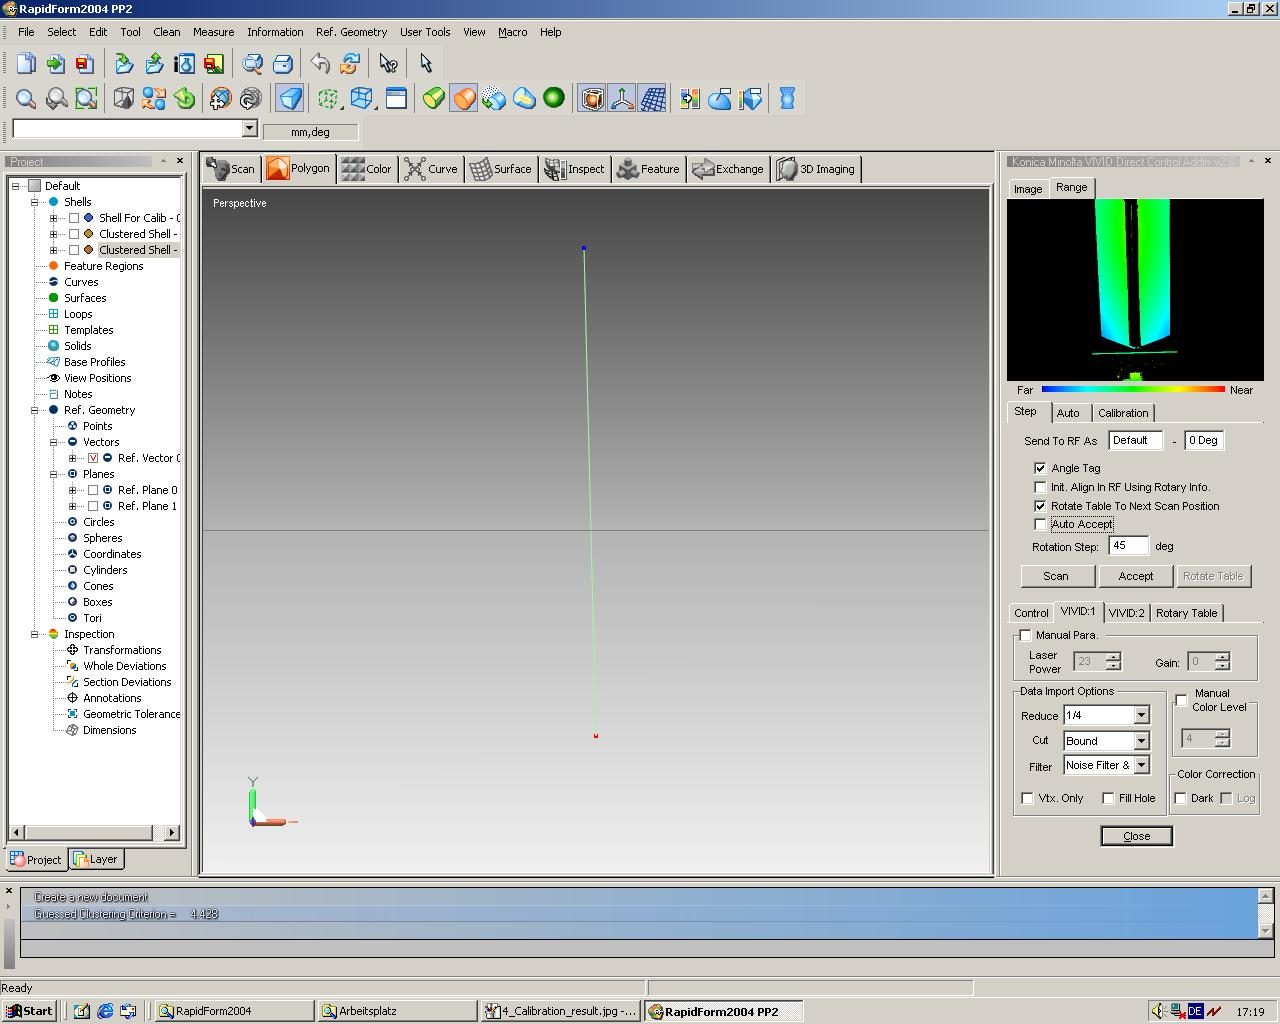
\includegraphics[width=8cm]{Anleitung/5_StepScan.jpg}
\\ \hline  

\multicolumn{2}{|l|}%
{{\textbf{Schritt 11 - AutoFocus}}}
\\ \hline
Das \emph{Kalibrationsblech} entfernen und durch das zu scannende Objekt ersetzen.\linebreak
Zum Reiter \textbf{Control} wechseln. \linebreak
Auf \textbf{Autofocus} klicken.\linebreak
& 
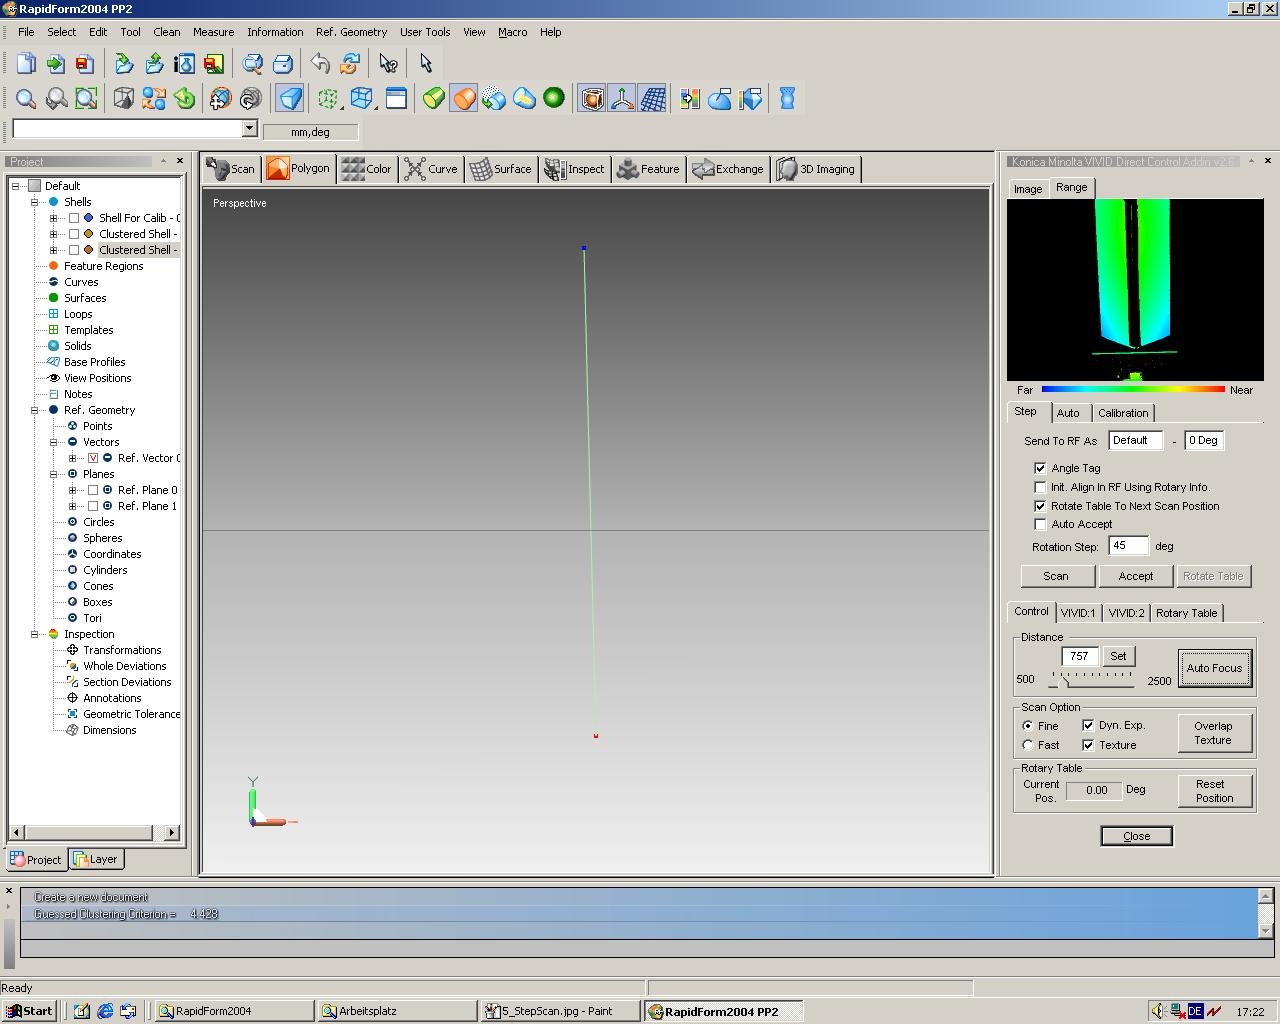
\includegraphics[width=8cm]{Anleitung/6_AutoFocus}
\\ \hline  

\multicolumn{2}{|l|}%
{{\textbf{Schritt 12 - Scan}}}
\\ \hline
Auf \textbf{Scan} klicken. \linebreak
Das Objekt sollte möglichst schon zu erkennen sein und die Farben sich im Mittleren Bereich bewegen. \linebreak
Ansonsten muss mit den Parametern \textbf{Focus} und \textbf{LaserPower gespielt werden.}
\begin{TippS}Die Position des VI-900 darf nach der Kalibrierung nicht mehr verändert werden!\end{TippS}
& 
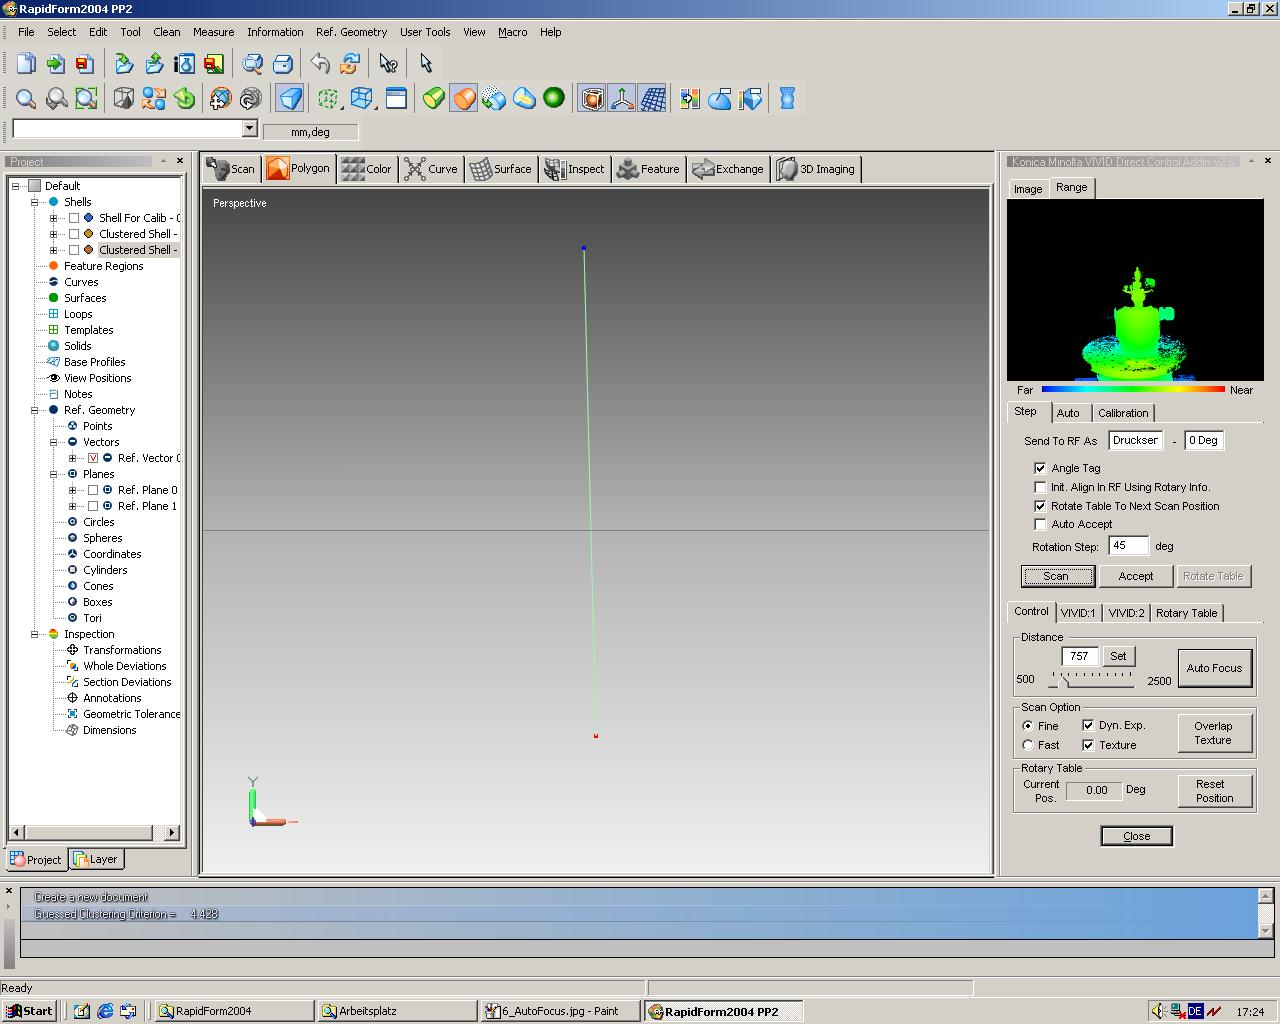
\includegraphics[width=8cm]{Anleitung/7_Scan}
\\ \hline  

\multicolumn{2}{|l|}%
{{\textbf{Schritt 13 - Akzeptieren}}}
\\ \hline
Ist das Objekt gut zu erkennen, können mit \textbf{Accept} die Daten an RapidForm2004 gesendet werden. Der Drehtisch sollte sich nun automatisch um den eingestellten Winkel drehen. 
\begin{TippS}Bei \textbf{AutoAccept} kann nun ein Häkchen gesetzt werden.\end{TippS}
& 
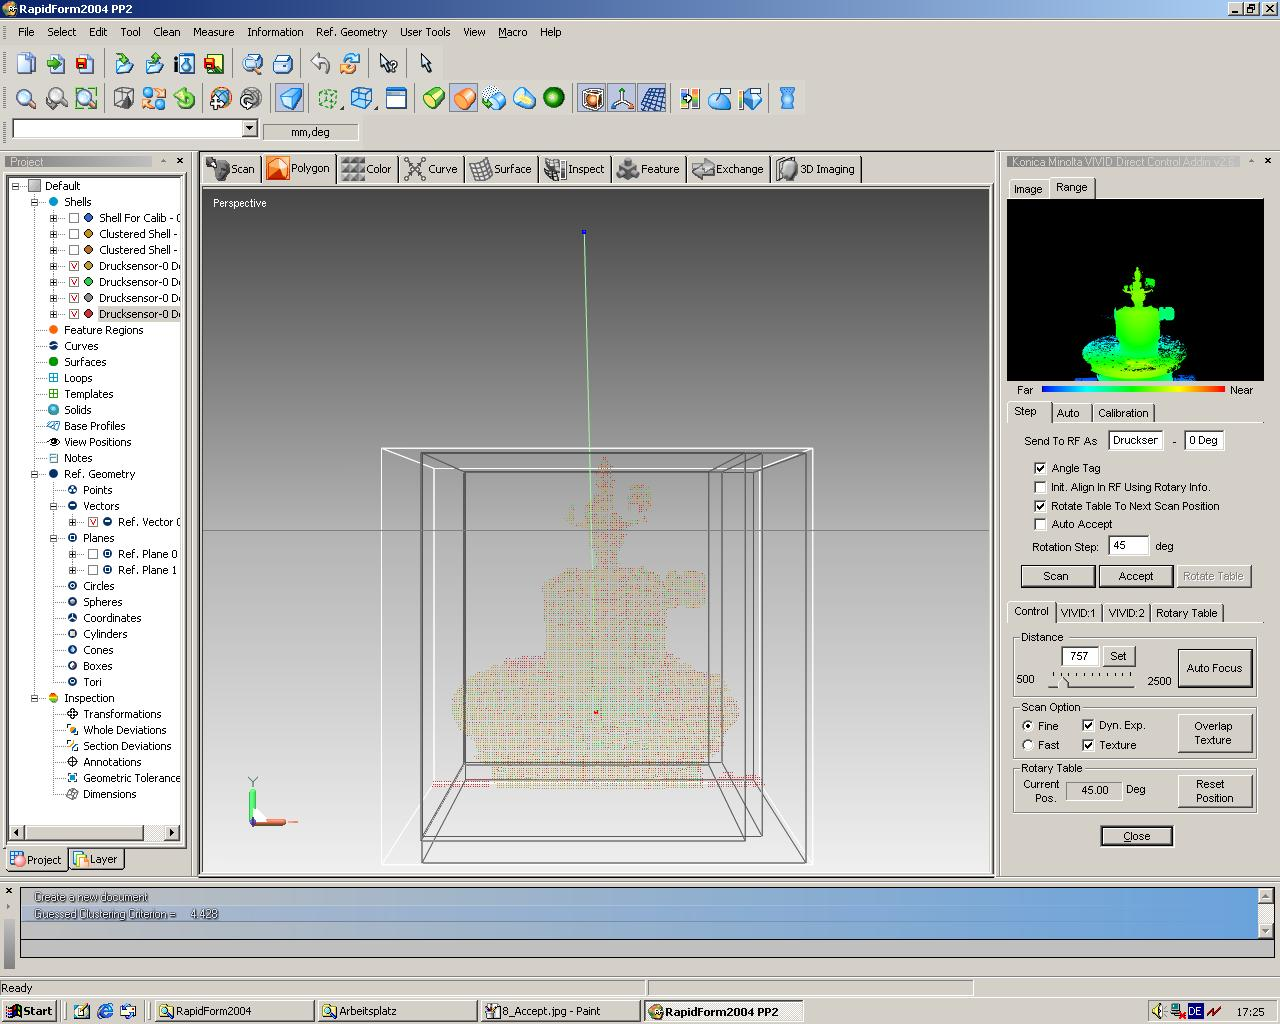
\includegraphics[width=8cm]{Anleitung/8_Accept}
\\ \hline  

\multicolumn{2}{|l|}%
{{\textbf{Schritt 14 - Scannen}}}
\\ \hline
Auf \textbf{Scan} klicken und warten bis der Scan abgeschlossen ist und der Tisch sich gedreht hat.\linebreak
Diesen Schritt wiederholen bis alle Aufnahmen abgeschlossen sind.\linebreak
& 
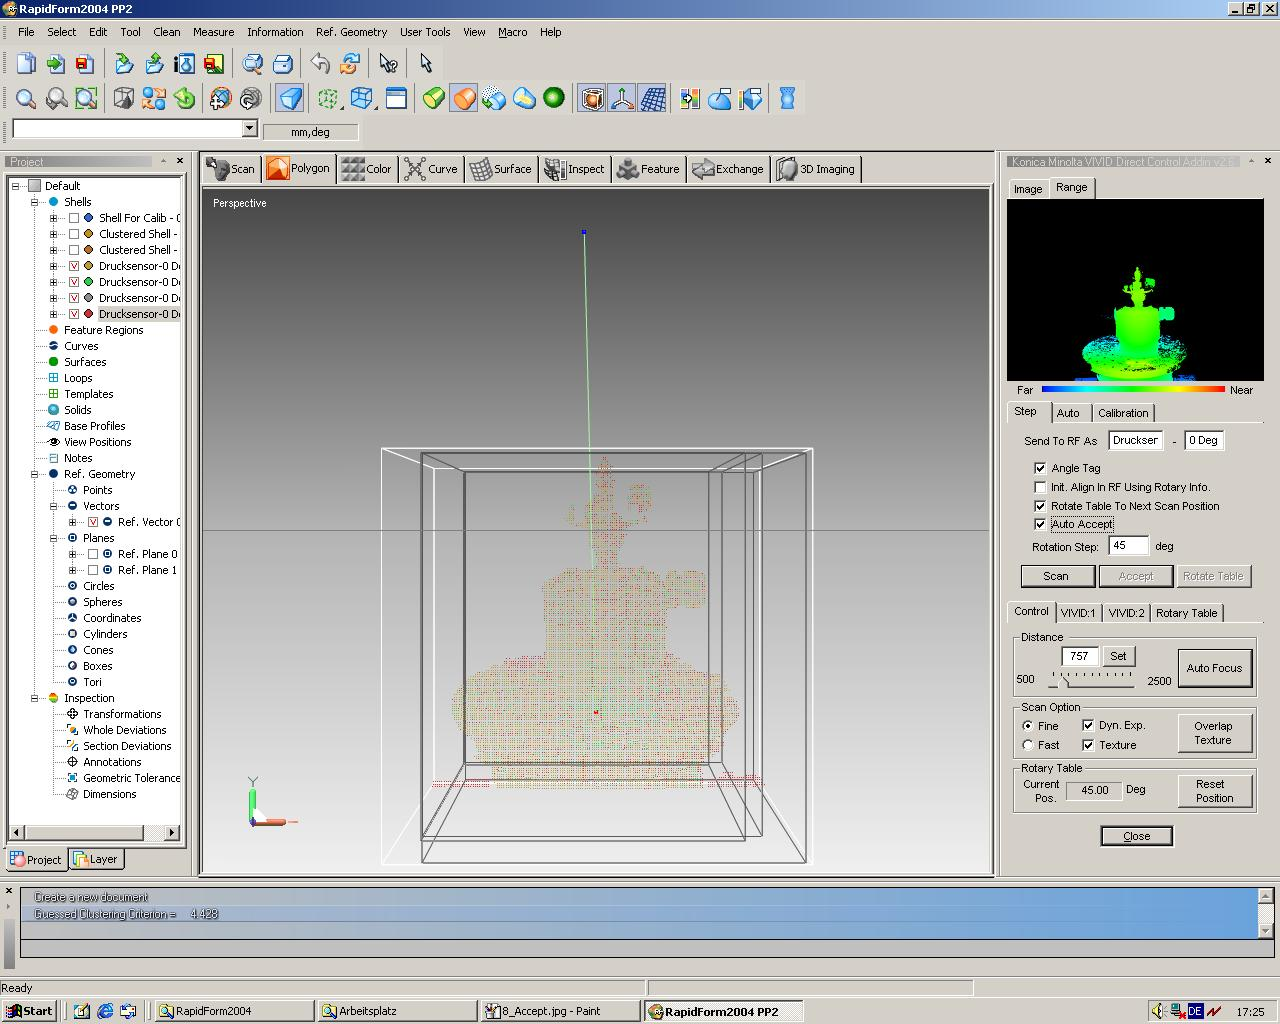
\includegraphics[width=8cm]{Anleitung/8_AutoAccept}
\\ \hline  

\multicolumn{2}{|l|}%
{{\textbf{Schritt 15 - Ergebnis der Scans}}}
\\ \hline
Nach Abschluss aller Scans dreht der Tisch sich automatisch in die Ursprungsposition zurück.\linebreak
Im Arbeitsbereich sollten sich nun alle Scans befinden.
& 
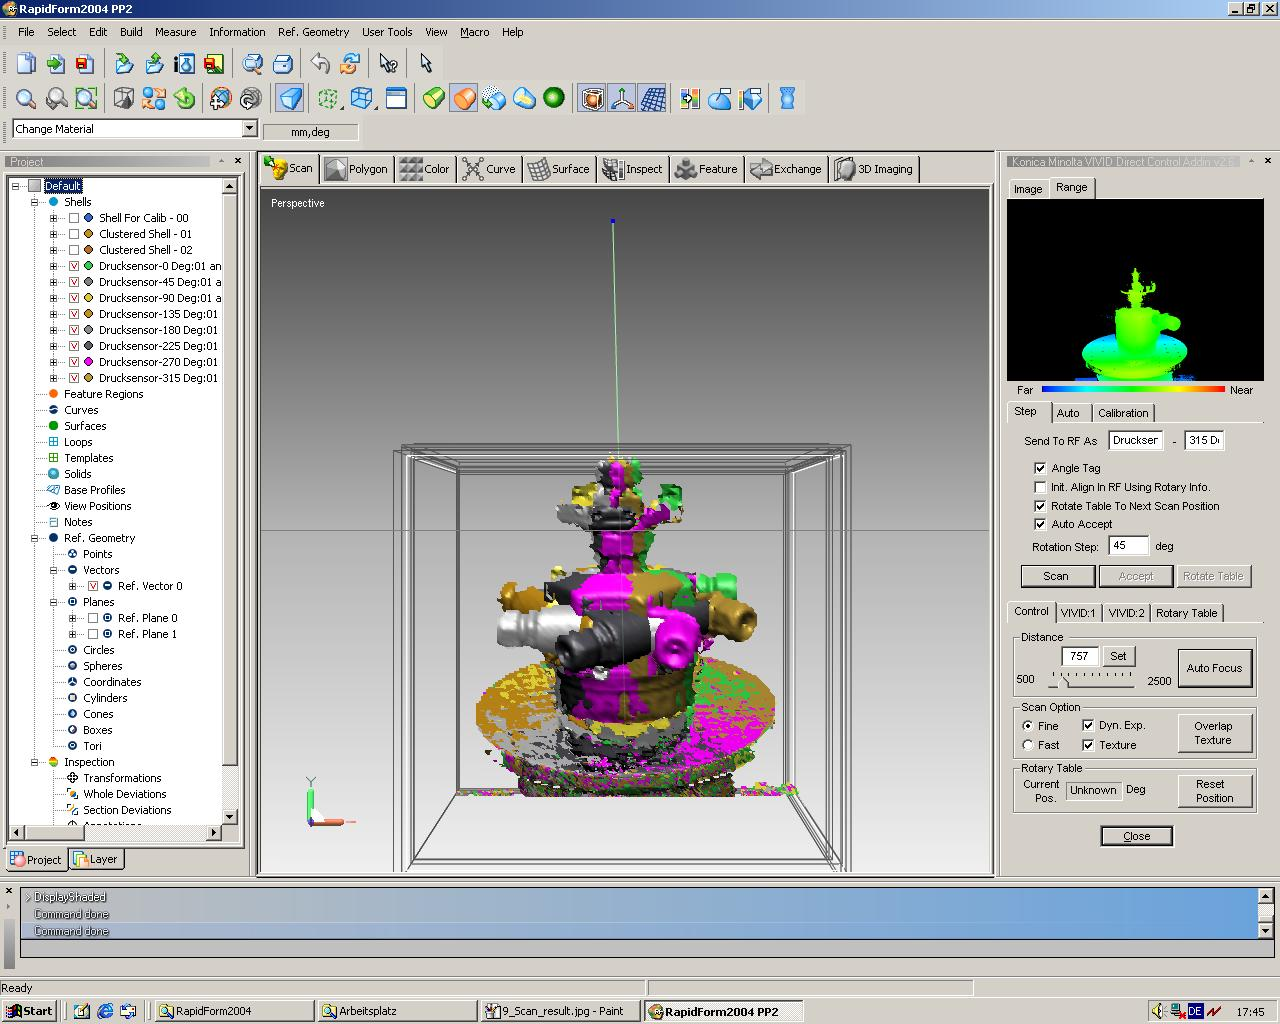
\includegraphics[width=8cm]{Anleitung/9_1_Scan_result}
\\ \hline  

\multicolumn{2}{|l|}%
{{\textbf{Schritt 16 - Drehen und Zusammenführen der Scans}}}
\\ \hline
In der Menüzeile auf \textbf{Build -> Register -> Rotary Table} klicken.\linebreak
& 
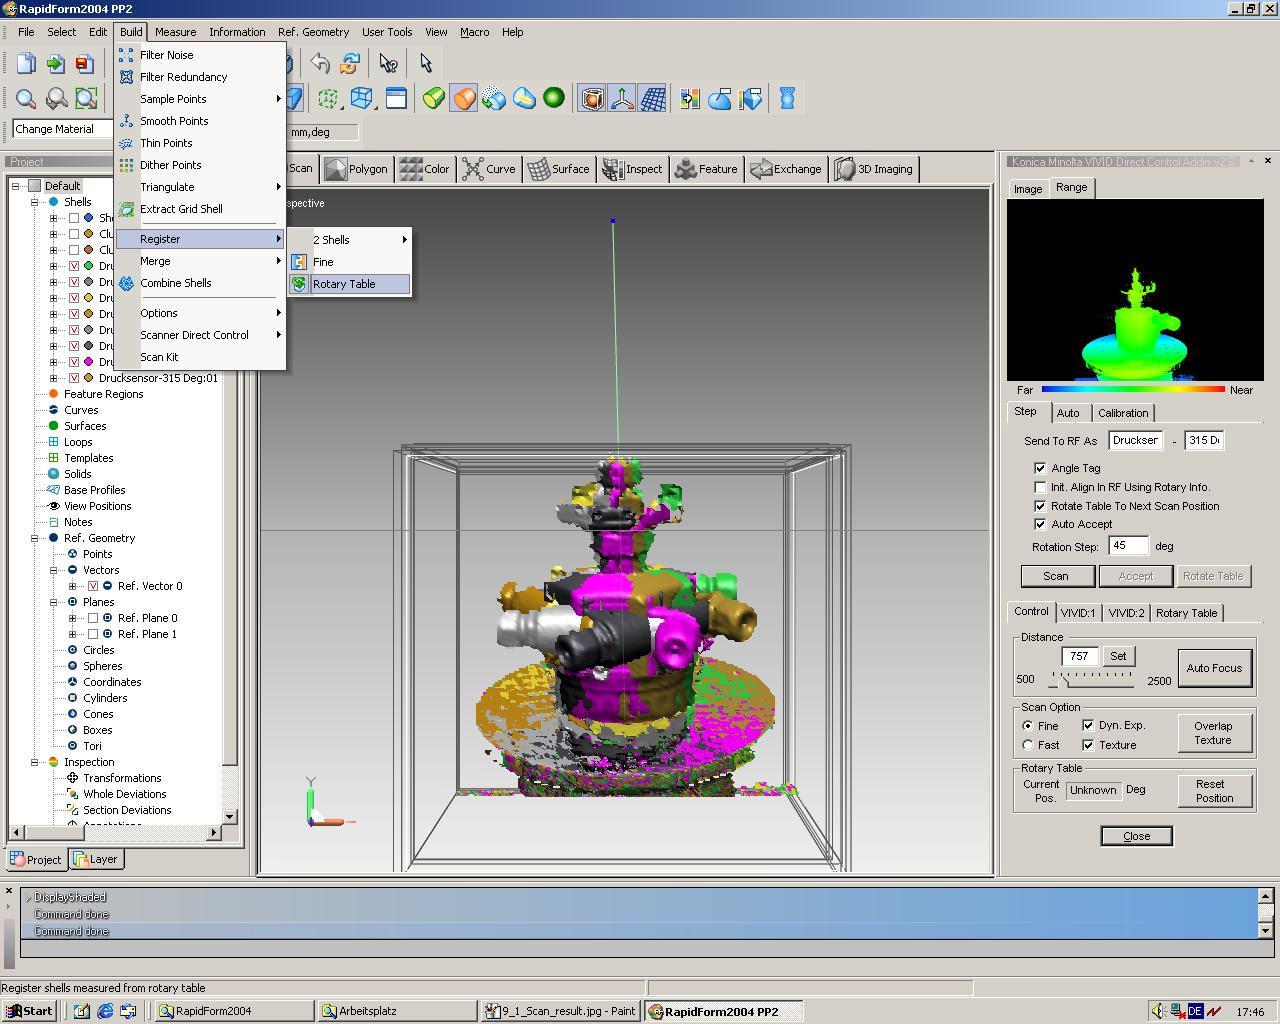
\includegraphics[width=8cm]{Anleitung/10_Rotary_Table}
\\ \hline  

\multicolumn{2}{|l|}%
{{\textbf{Schritt 17 - Registrieren}}}
\\ \hline
Im Dialog auf \textbf{Select Axis} klicken.\linebreak
Im Darstellungsbereich auf die Achse aus dem Kalibrationsscan klicken.
Bei \textbf{Rotation-Angle} den Winkel eines Scans eintragen.\linebreak
Im \emph{Projektbaum} den Entsprechenden Scan auswählen.\linebreak
Die letzten beiden Schritte mit allen Scans wiederholen.\linebreak
Den Dialog mit \textbf{Ok} verlassen.
& 
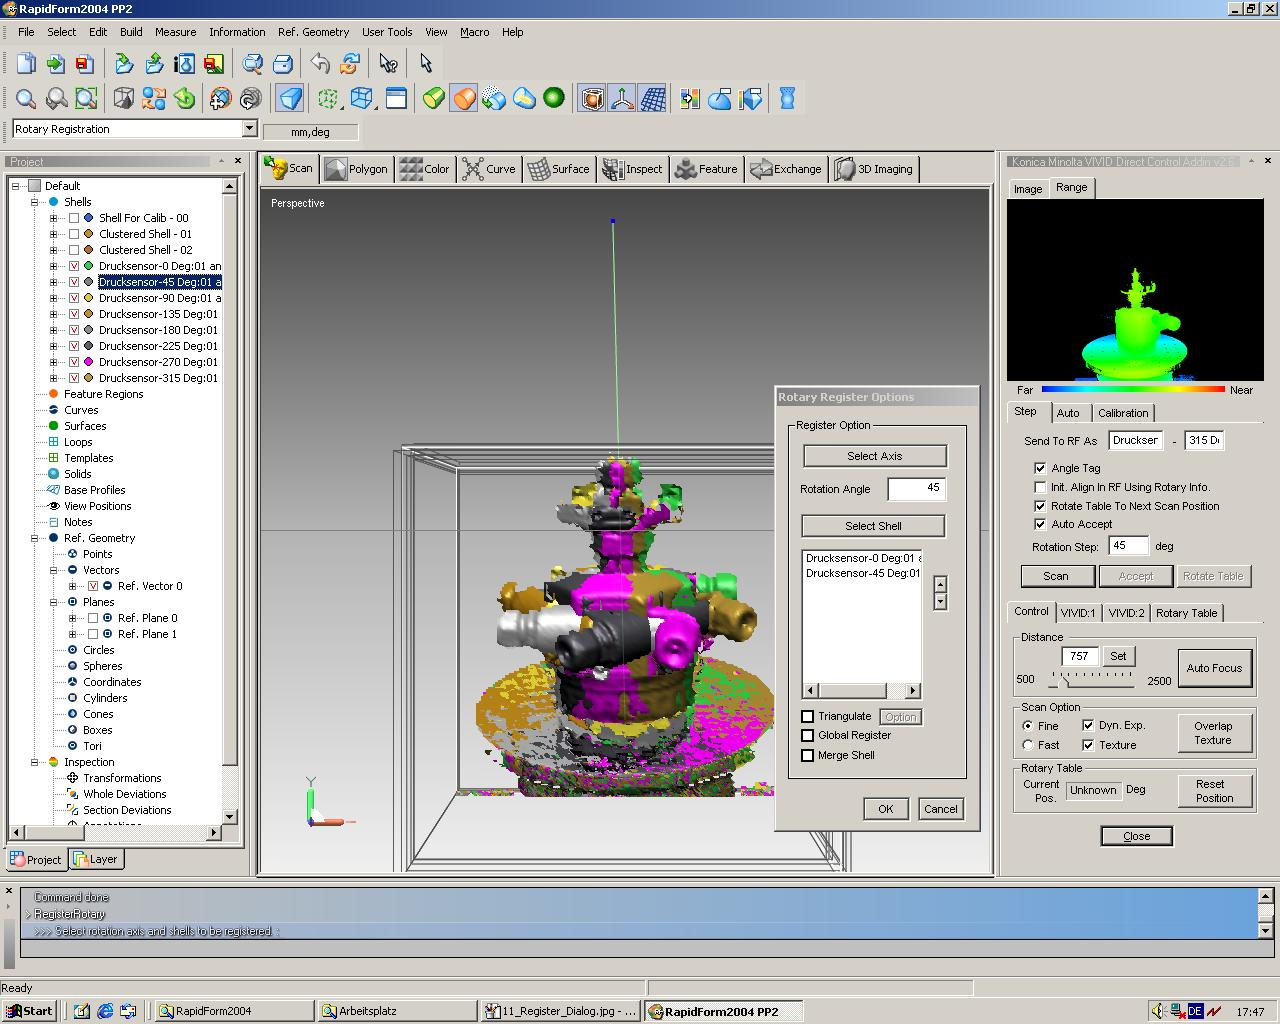
\includegraphics[width=8cm]{Anleitung/11_Register_Dialog_2}
\\ \hline  

\multicolumn{2}{|l|}%
{{\textbf{Schritt 18 - Ergebnis}}}
\\ \hline
Das Ergebnis ist ein komplettes 3D-Modell des Objektes.
& 
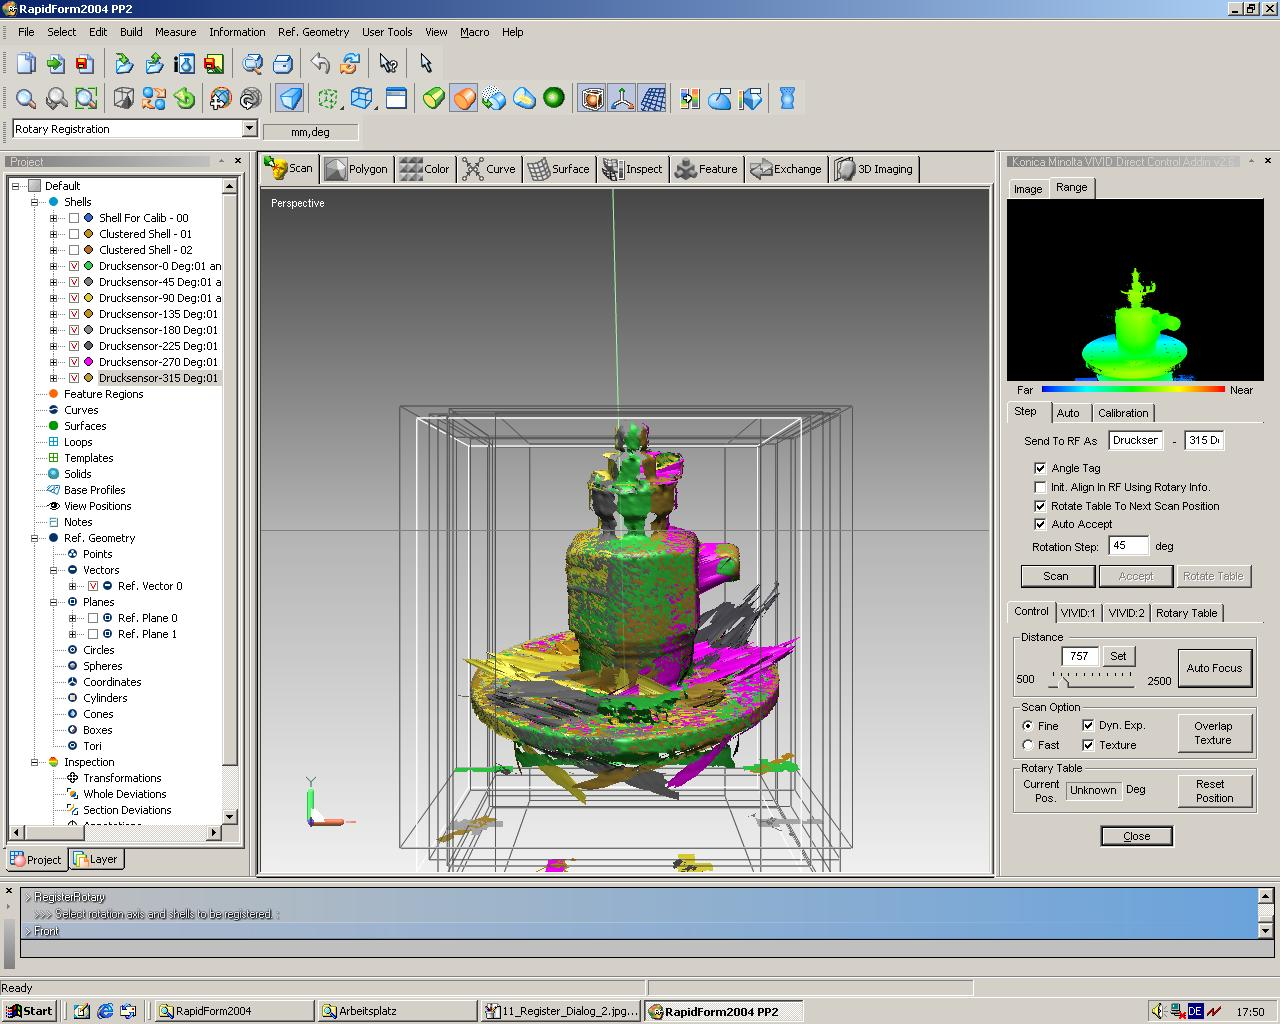
\includegraphics[width=8cm]{Anleitung/11_Register_result}
\\ \hline  

\end{longtable} 

\section{Technische Daten VI-910}
Die Technischen Daten beziehen sich auf den VI-910. Dies ist das Nachfolgemodell. Die meisten Daten sollten jedoch ähnlich sein.
\begin{longtable}{|m{4cm}|m{9cm}|} 
\caption{Technische Daten - VI-910} \\
\hline
\label{tab:TD_VI-910}
Modellbezeichnung & Optischer 3D-Scanner VI-910
 \\ \hline 
Messverfahren & Triangulation durch Lichtschnittverfahren
 \\ \hline 
Autofokus & Autofokus auf Objektoberfläche (Kontrastverfahren);  aktiver AF
 \\ \hline 
Objektive \newline  (wechselbar) & TELE Brennweite f=25mm  \newline 
MITTEL: Brennweite f=14 mm  \newline 
WEIT: Brennweite f=8mm
 \\ \hline 
Messabstand & 0,6 bis 2,5m (2m für WIDE-Objektiv)
 \\ \hline 
Optimaler Messabstand	 & 0,6 bis 1,2m
 \\ \hline 
Laserklasse & Class 2 (IEC60825-1), Class 1 (FDA)
 \\ \hline 
Laser-Scanverfahren	 & Galvanisch-angetriebener Drehspiegel
 \\ \hline 
Messbereich in  \newline X-Richtung (anhängig vom Anstand) & 111 bis 463mm (TELE),  \newline 198 bis 823mm (MITTEL), \newline  359 bis 1.196mm (WEIT)
 \\ \hline 
Messbereich in Y-Richtung (abhängig vom Abstand) & 83 bis 347mm (TELE), \newline  148 bis 618mm (MITTEL),  \newline 269 bis 897mm (WEIT)
 \\ \hline 
Messbereich in Z-Richtung (abhängig vom Abstand) & 40 bis 500mm (TELE), \newline  70 bis 800mm (MITTEL),  \newline 110 bis 750mm (WEIT/Modus FINE)
 \\ \hline 
Genauigkeit	 & X: ±0,22mm, Y: ±0,16mm, Z: ±0,10mm zur Z-Referenzebene (Bedingungen: TELE/Modus FINE , Konica Minolta Standard)
 \\ \hline 
Aufnahmezeit & 0,3s (Modus FAST), 2,5s (Modus FINE), 0,5s (COLOR)
 \\ \hline 
Übertragungszeit zum Host-Computer	 & ca. 1s (Modus FAST) oder 1,5s (Modus FINE)
 \\ \hline 
Scanumgebung, Beleuchtungsbedingungen	 & 500 lx oder geringer
 \\ \hline 
Aufnahmeeinheit & 3D-Daten: 1/3" CCD-Bildsensor (340.000 Pixel) 
Farbdaten: Zusammen mit 3D-Daten (Farbtrennung durch Drehfilter)
 \\ \hline 
Anzahl aufgenommener Punkte	 & 3D-Daten: 307.000 (Modus FINE), 76.800 (Modus FAST) 
Farbdaten: 640 × 480 × 24 Bit Farbtiefe
 \\ \hline 
Ausgabeformat & 3D-Daten: Konica Minolta Format, (STL, DXF, OBJ, ASCII-Punkte, VRML; Konvertierung in 3D-Daten durch Polygon Editing-Software / Standardzubehör)
Farbdaten: RGB 24-Bit Rasterscan-Daten
 \\ \hline 
Speichermedium & Compact Flash Memory Card (128MB)
 \\ \hline 
Dateigrößen & 3D- und Farbdaten (kombiniert): 1,6MB (Modus FAST) pro Datensatz, 3,6MB (Modus FINE) pro Datensatz 
 \\ \hline 
Monitor & 5,7"-LCD (320 × 240 Pixel)
 \\ \hline 
Datenschnittstelle & SCSI II (DMA-Synchronübertragung)
 \\ \hline 
Stromversorgung & Normale Wechselstromversorgung, 100V bis 240 V (50 oder 60 Hz), Nennstrom 0,6 A (bei 100 V) \\ \hline 
Abmessungen (B x H x T)	 & 213 × 413 × 271mm 
 \\ \hline 
Gewicht & ca. 11kg
 \\ \hline 
Zulässige Umgebungsbedingungen (Betrieb) & 10 bis 40°C; relative Luftfeuchtigkeit 65\% oder niedriger (keine Kondensation)
 \\ \hline 
Zulässige Umgebungsbedingungen (Lagerung) & -10 bis 50°C, relative Luftfeuchtigkeit 85\% oder niedriger (bei 35°C, keine Kondensation) 
 \\ \hline 
\end{longtable} 
%\include{Inhalt/uCGrundlagen}
%\include{Inhalt/RS232Grundlagen}
\section{Vom Autor verwendete Software}
\label{sec:Werkzeuge}
Hier ist die verwendete Software aufgelistet. Soweit es möglich war, wurden Open-Source-Programme eingesetzt.
\todo{Überarbeiten!!!}
\begin{itemize}
\item \textbf{RapidForm2004} \\
asdf
\item \textbf{AVRStudio 5} \\
Atmel. \\
Website: \url{http://www.atmel.com/}  
\item \textbf{Eclipse} \\
Eclipse mit CDT und AVRPlugin
\\
Website: \url{http://www.eclipse.org/}  
\item \textbf{AVRDude} \\
Prorammer \\
\todo{Weitere?!}
\end{itemize}

%\section{Codelistings}
%Die ungekürzten Sourcecodes.
\section{main.c}
\label{sec:main.c}
\lstset{language=C, basicstyle=\footnotesize, showstringspaces=false, tabsize=4, inputencoding={utf8}}
\lstinputlisting[label=lst:main,caption=main.c]{../../main.c}
%\subsection{lcd.h}
%\lstset{language=Java, basicstyle=\footnotesize, showstringspaces=C, tabsize=4}
%\lstinputlisting[label=lst:lcd.h,caption=lcd.h]{../../lcd.h}
%\subsection{Debounce.h}
%\lstset{language=C, basicstyle=\footnotesize, showstringspaces=false, tabsize=4}
%\lstinputlisting[label=lst:Debounce.h,caption=Debounce.h]{../../lcd.h}
%\subsection{tinymenu.h}
%\subsection{mymenu.h}
%\subsection{mystuff.h}
%\include{Inhalt/Danksagung} %Vorlage, C-B, Bildh, Werkstatt, Steimers und Co.
\end{appendix}


% Index --------------------------------------------------------------------
%	Zum Erstellen eines Index, die folgende Zeile auskommentieren.
% --------------------------------------------------------------------------
\printindex		% Index hier einfügen

\end{document}
